 %	Main Document

\documentclass[
	12pt,
	BCOR=5mm,
	DIV=12,
	headinclude=on,
	footinclude=off,
	parskip=half,
	bibliography=totoc,
	listof=entryprefix,
	toc=listof,
	pointlessnumbers,
	plainfootsepline]{scrreprt}

% include configuration file
% !TEX root =  master.tex

% language, font, colors
\usepackage[ngerman]{babel}
\usepackage[utf8]{inputenc}
\usepackage[german=quotes]{csquotes} 	% correct quotes using \enquote{}
\usepackage[T1]{fontenc}
\usepackage{lmodern} % latin modern font, TODO: Arial 12?
\usepackage[onehalfspacing]{setspace}
\usepackage{xcolor}

% hyperlinks
\usepackage[hidelinks=true]{hyperref}

% commands for author and title
\newcommand{\TitelDerArbeit}[1]{\def\DerTitelDerArbeit{#1}\hypersetup{pdftitle={#1}}}
\newcommand{\AutorDerArbeit}[1]{\def\DerAutorDerArbeit{#1}\hypersetup{pdfauthor={#1}}}
\newcommand{\Firma}[1]{\def\DerNameDerFirma{#1}}
\newcommand{\Kurs}[1]{\def\DieKursbezeichnung{#1}}

%\usepackage{microtype}% verbesserter Randausgleich
%\setlength\emergencystretch{1em}
% correct superscripts 
\usepackage{fnpct}

\usepackage{footnote}
\usepackage{rotating} 

% calc 
\usepackage{calc} % Used for extra space below footsepline

% bibliography settings
% author-year-style with footnotes (Chicago)
\usepackage[backend=biber, autocite=footnote, style=authoryear, dashed=false]{biblatex}
\AdaptNoteOpt\footcite\multfootcite
\AdaptNoteOpt\autocite\multautocite

\DefineBibliographyStrings{ngerman}{  % change u.a. to et al. (german only!)
	andothers = {{et\,al\adddot}},
}
% Command to output section title headings
\newcommand{\cvsect}[1]{% The only parameter is the section text
	\vspace{\baselineskip} % Whitespace before the section title
	\colorbox{black}{\textcolor{white}{\MakeUppercase{\textbf{#1}}}}\\% Section title
}

\usepackage{longtable} % Required for tables that span multiple pages
\setlength{\LTpre}{0pt} % Remove default whitespace before longtable
\setlength{\LTpost}{0pt} % Remove default whitespace after longtable

\setlength{\tabcolsep}{0pt} % No spacing between table columns

% Environment to hold a new list of entries
\newenvironment{entrylist}{
	\begin{longtable}[H]{l l}
	}{
	\end{longtable}
}

\newcommand{\entry}[2]{% First argument for the leftmost date(s) text, second is for the entry heading
	\vspace{-0.15cm}
	\parbox[t]{0.33\textwidth}{% 25.0% of the text width of the page
		#1 % Leftmost entry date(s) text
	}%
	&\parbox[t]{0.68\textwidth}{% 75.0% of the text width of the page
		{#2}% Entry heading text
	}\\\\}

\newcounter{barcount}

% Environment to hold a new bar chart
\newenvironment{barchart}[1]{ % The only parameter is the maximum bar width, in cm
	\newcommand{\barwidth}{0.35}
	\newcommand{\barsep}{0.55}
	
	% Command to add a bar to the bar chart
	\newcommand{\baritem}[2]{ % The first argument is the bar label and the second is the percentage the current bar should take up of the total width
		\pgfmathparse{##2}
		\let\perc\pgfmathresult
		
		\pgfmathparse{#1}
		\let\barsize\pgfmathresult
		
		\pgfmathparse{\barsize*##2/5}
		\let\barone\pgfmathresult
		
		\pgfmathparse{(\barwidth*\thebarcount)+(\barsep*\thebarcount)}
		\let\barx\pgfmathresult
		
		\filldraw[fill=none, draw=black!] (0,-\barx) rectangle (5,-\barx-\barwidth);
		\filldraw[fill=black!90, draw=black!90] (0,-\barx) rectangle (\barone,-\barx-\barwidth);
		
		\node [label=180:{\textcolor{black}{##1: ##2/5}}] at (0,-\barx-0.175) {};
		\addtocounter{barcount}{1}
	}
	\begin{tikzpicture}
	\setcounter{barcount}{0}
}{
	\end{tikzpicture}
	\vspace{0.3cm}
}

\usepackage{tikz} % Required for creating the plots
\usetikzlibrary{shapes, backgrounds}
\tikzset{x=1cm, y=1cm} % Default tikz units

%%% Uncomment the following lines to support hard URL breaks in bibliography 
%\apptocmd{\UrlBreaks}{\do\f\do\m}{}{}
%\setcounter{biburllcpenalty}{9000}% Kleinbuchstaben
%\setcounter{biburlucpenalty}{9000}% Großbuchstaben

\setlength{\bibparsep}{\parskip}	% add some space between biblatex entries in the bibliography
\addbibresource{bibliography.bib}	% add file bibliography.bib as biblatex resource

% footnotes (count footnotes over chapters)
\usepackage{chngcntr}
\counterwithout{footnote}{chapter}

% acronyms
\makeatletter
\usepackage[printonlyused]{acronym}
\@ifpackagelater{acronym}{2015/03/20}
  {%
    \renewcommand*{\aclabelfont}[1]{\textbf{\textsf{\acsfont{#1}}}}
  }%
  {%
  }%
\makeatother

% listings
\usepackage{listings}
\renewcommand{\lstlistingname}{Quelltext} 
\renewcommand{\lstlistlistingname}{Quelltextverzeichnis}

%% More configuration for listings is in configlistings.tex %%


% extra packages
\usepackage{graphicx}			% use various graphics formats
\usepackage{subfig}				% sub-figures, e.g. side-by-side pictures
\usepackage[german]{varioref}	% nicer references \vref
\usepackage{caption}			% better captions
\usepackage{booktabs}			% nicer tabs
\usepackage{array}

% algorithms
\usepackage{algorithm}
\usepackage{algpseudocode}
\renewcommand{\listalgorithmname}{Algorithmenverzeichnis}
\floatname{algorithm}{Algorithmus}

% page header/footer
\RequirePackage[automark,headsepline,footsepline]{scrpage2}
\pagestyle{scrheadings}
\renewcommand*{\pnumfont}{\upshape\sffamily}
\renewcommand*{\headfont}{\upshape\sffamily}
\renewcommand*{\footfont}{\upshape\sffamily}
\renewcommand{\chaptermarkformat}{}
\RedeclareSectionCommand[beforeskip=0pt]{chapter}
\clearscrheadfoot

\ifoot[\rule{0pt}{\ht\strutbox+\dp\strutbox}DHBW Mannheim]{\rule{0pt}{\ht\strutbox+\dp\strutbox}DHBW Mannheim}
\ofoot[\rule{0pt}{\ht\strutbox+\dp\strutbox}\pagemark]{\rule{0pt}{\ht\strutbox+\dp\strutbox}\pagemark}

\ohead{\headmark}

% !TEX root =  master.tex

% colors
\definecolor{javared}{rgb}{0.6,0,0} % for strings
\definecolor{javagreen}{rgb}{0.25,0.5,0.35} % comments
\definecolor{javapurple}{rgb}{0.5,0,0.35} % keywords
\definecolor{javadocblue}{rgb}{0.25,0.35,0.75} % javadoc

\colorlet{jsonPunct}{red!60!black}
\definecolor{jsonBackground}{HTML}{EEEEEE}
\definecolor{jsonDelim}{RGB}{20,105,176}
\colorlet{jsonNumb}{magenta!60!black}

\definecolor{xmlGray}{rgb}{0.4,0.4,0.4}
\definecolor{xmlDarkblue}{rgb}{0.0,0.0,0.6}
\definecolor{xmlCyan}{rgb}{0.0,0.6,0.6}

\definecolor{jsBackground}{RGB}{250,250,255}
\definecolor{jsString}    {RGB}{ 16,160, 60}

\definecolor{cssKeyword}{RGB}{ 10,100,160}
\definecolor{cssClass}  {RGB}{200,120, 10}

% general style
\lstset{
	basicstyle=\ttfamily\footnotesize,
	backgroundcolor=\color{jsBackground},
	numbers=left,
	numberstyle=\scriptsize\color{black},
	stepnumber=1,
	numbersep=10pt,
	showspaces=false,
	showstringspaces=false,
	breaklines=true,
	tabsize=2,
	captionpos=b,
	literate=
	{Ö}{{\"O}}1
	{Ä}{{\"A}}1
	{Ü}{{\"U}}1
	{ß}{{\ss}}1
	{ü}{{\"u}}1
	{ä}{{\"a}}1
	{ö}{{\"o}}1
}

% Java
\lstdefinestyle{lstJava}
{
	language=Java,
	keywordstyle=\color{javapurple}\bfseries,
	stringstyle=\color{javared},
	commentstyle=\color{javagreen},
	morecomment=[s][\color{javadocblue}]{/**}{*/},
	tabsize=1
}

% JSON
\lstdefinelanguage{json}{
	frame=lines,
	backgroundcolor=\color{jsonBackground},
	literate=
	*{0}{{{\color{jsonNumb}0}}}{1}
	{1}{{{\color{jsonNumb}1}}}{1}
	{2}{{{\color{jsonNumb}2}}}{1}
	{3}{{{\color{jsonNumb}3}}}{1}
	{4}{{{\color{jsonNumb}4}}}{1}
	{5}{{{\color{jsonNumb}5}}}{1}
	{6}{{{\color{jsonNumb}6}}}{1}
	{7}{{{\color{jsonNumb}7}}}{1}
	{8}{{{\color{jsonNumb}8}}}{1}
	{9}{{{\color{jsonNumb}9}}}{1}
	{:}{{{\color{jsonPunct}{:}}}}{1}
	{,}{{{\color{jsonPunct}{,}}}}{1}
	{\{}{{{\color{jsonDelim}{\{}}}}{1}
	{\}}{{{\color{jsonDelim}{\}}}}}{1}
	{[}{{{\color{jsonDelim}{[}}}}{1}
	{]}{{{\color{jsonDelim}{]}}}}{1}
}

% XML
\lstdefinelanguage{XML}
{
	morestring=[b]",
	morestring=[s]{>}{<},
	morecomment=[s]{<?}{?>},
	stringstyle=\color{xmlGray},
	identifierstyle=\color{xmlDarkblue},
	keywordstyle=\color{xmlCyan},
	morekeywords={xmlns,version,type}
}

% JavaScript
\lstdefinelanguage{JavaScript}
{
	backgroundcolor=\color{jsBackground},
	keywordstyle=\color{blue}\bfseries,
	stringstyle=\color{jsString},
	commentstyle=\color{gray},
	morestring=[b]",
	morecomment=[l][\color{gray}]{//},
	morecomment=[s][\color{gray}]{/*}{*/},
	morekeywords={break,case,const,continue,else,false,for,function,if,in,new,null,switch,this,true,var,while}
}

% HTML
\lstdefinestyle{lstHTML}
{
	language=HTML,
	keywordstyle=\color{blue}\bfseries,
	commentstyle=\color{gray}\itshape,
	morecomment=[s][\color{gray}]{<!--}{-->},
%	stringstyle=\color{jsString}
	escapeinside=``
}

% CSS
\lstdefinestyle{lstCSS}
{
	keywordstyle=\color{cssKeyword}\bfseries,
	commentstyle=\color{gray}\itshape,
	morecomment=[s][\color{gray}]{/*}{*/},
%	morecomment=[s][\color{cssClass}]{.}{ \{},
	alsoletter=-,
	morekeywords={border,background-color}
}

% !TEX root =  master.tex

\newcommand{\authorSG}{Sascha Görnert}
\newcommand{\authorNL}{Niko Lockenvitz}
\newcommand{\authorRF}{Rene Fischer}
\newcommand{\authorEJ}{Erik Jansky}
\newcommand{\authorGP}{Gerrit Pollkläsener}

\begin{document}

% set some information (title, author, ...)
\TitelDerArbeit{Entwurf und Implementierung eines Kinoreservierungssystems}
\AutorDerArbeit{\authorSG, \authorRF, \authorGP, \authorEJ, \authorNL}
\Firma{DER Touristik GmbH, Technische Universität Kaiserslautern, SAP SE}
\Kurs{WWI 17 SE B}

\begin{titlepage}

\begin{minipage}{\textwidth}
	\vspace{-2cm}
	\noindent
	
\includegraphics[height=0.1\linewidth]{img/logos/der}
	\hfill
	
\includegraphics[height=0.1\linewidth]{img/logos/tukl}
	\hfill
	
\includegraphics[height=0.1\linewidth]{img/logos/sap}
	\hfill
	
\includegraphics[height=0.1\linewidth]{img/logos/dhbw}
\end{minipage}

\vspace{1em}
\sffamily

\begin{center}
	\textsf{\large{}Duale Hochschule Baden-Württemberg\\[1.5mm] Mannheim}\\[2em]
	\textsf{\textbf{\Large{}Seminararbeit}}\\[3mm]
	\textsf{\textbf{\DerTitelDerArbeit}}\\[1.5cm]
	\textsf{\textbf{\Large{}Studiengang Wirtschaftsinformatik}\\[3mm] \textsf{Studienrichtung Software Engineering}}
	
	\vspace{3em}
	\vfill

	\begin{minipage}{\textwidth}
	
		\begin{tabbing}
			Bearbeitungszeitraum: \hspace{0.85cm}\=\kill
			Verfasser: \> Sascha Görnert, 2716910 \\
			\> DER Touristik GmbH \\
			\> \\
			\> Rene Fischer, 8703049 \\
			\> Technische Universität Kaiserslautern \\
			\> \\
			\> Gerrit Pollkläsener, 1930724 \\
			\> SAP SE \\
			\> \\
			\> Erik Jansky, 5980253 \\
			\> SAP SE \\
			\> \\
			\> Niko Lockenvitz, 1308674 \\
			\> SAP SE \\
			\> \\[1.5mm]
			Kurs: \> \DieKursbezeichnung \\[1.5mm]
			Bearbeitungszeitraum: \> 19.11.2018 -- 12.02.2019
	\end{tabbing}

	\end{minipage}

\end{center}

\end{titlepage}

\pagenumbering{roman}
\normalfont

% abstract
\chapter*{Kurzfassung}
\begingroup
\begin{table}[h!]
\setlength\tabcolsep{0pt}
\begin{tabular}{p{3.7cm}p{11.7cm}}
Titel & \DerTitelDerArbeit \\
Verfasser: & \DerAutorDerArbeit \\
Kurs: & \DieKursbezeichnung \\
\end{tabular}
\end{table}
\endgroup

Zusammenfassung der Arbeit

% table of contents
\tableofcontents

% figures
\listoffigures

% tables
%\listoftables

% listings (source code)
\lstlistoflistings

% acronyms
\clearpage
\chapter*{Abkürzungsverzeichnis}
\addcontentsline{toc}{chapter}{Abkürzungsverzeichnis}

\begin{acronym}[A23456789012] % longest acronym for correct indentation
	\acro{A23456789012}{This is just for indentation}

	\acro{AJAX}{Asynchronous JavaScript and XML}
	\acro{API}{Application Programming Interface}
	\acro{CRUD}{CREATE, READ, UPDATE, DELETE}
	\acro{CSS}{Cascading Style Sheets}
	\acro{DAO}{Data Access Object}
	\acro{DBMS}{Datenbankmanagementsystem}
	\acro{DOM}{Document Object Model}
	\acro{DTO}{Data Transfer Object}
	\acro{ER-Modell}{Entity-Relationship-Modell}
	\acro{HTML}{Hypertext Markup Language}
	\acro{HTTP}{Hypertext Transfer Protocol}
	\acro{HTTPS}{Hypertext Transfer Protocol Secure}
	\acro{IDE}{Integrated Development Environment}
	\acro{JPA}{Java Persistence API}
	\acro{JPQL}{Java Persistence Query Language}
	\acro{JSON}{JavaScript Object Notation}
	\acro{ORM}{Objektrelationaler Mapper}
	\acrodefplural{ORM}{Objectrelationale Mapper}
	\acro{POJO}{Plain Old Java Object}
	\acro{REST}{Representational State Transfer}
	\acro{SQL}{Structured Query Language}
	\acro{URI}{Uniform Resource Identifier}
	\acro{URL}{Uniform Resource Locator}
\end{acronym}

\ohead{Acronyms}

%--------------------------------
% Content
%--------------------------------
\clearpage
\ihead{\chaptername~\thechapter}
\ohead{\headmark}
\pagenumbering{arabic}

% one file for each chapter
% !TEX root =  master.tex
\chapter{Einleitung}

Diese Seminararbeit beschreibt das im Umfang des Moduls Fallstudie entwickelte Kinoreservierungssystem der Gruppe um Sascha Görnert, Rene Fischer, Erik Jansky, Niko Lockenvitz und Gerrit Pollkläsener.
Zielsetzung des zu entwickelten Systems ist es, einem Nutzer die Online-Buchung eines (oder mehrerer) Kinotickets zu ermöglichen.
Eine genauere Erläuterung der eigens gesetzten Ziele sowie eine Betrachtung, inwiefern diese erreicht wurden, findet in Kapitel \vref{sec:ziele} statt.
In den folgenden Abschnitten werden die durchlaufenen Entwicklungsschritte, einschließlich Planungsphase, Umsetzung und Reflexion erläutert und spezifiziert.

% !TEX root =  master.tex
\chapter{Analyse}
\chaptermulitpleauthor{\authorSG}{\authorGP, \authorRF, \authorEJ}

% !TEX root =  master.tex
\section{Personas}

In der Analysephase wurden folgende Personas erstellt:
\begin{enumerate}
\item Johnny Cash
\item Leon Schweickert
\item Florentina Kastenkette
\item Familie Mandick
\item Oma Gertrud
\end{enumerate}
% !TEX root =  master.tex
\section{User-Stories}

Mit der großen Spannbreite an Personas gibt es auch zahlreiche, teils sich stark unterscheidende Anforderungen an das Kinobuchungssystem.
Im folgenden Abschnitt werden diese Wünsche der Personas aufgezählt und gruppiert.

\subsection{Übersicht / Filmauswahl}
Zuerst werden die Anforderungen an eine Übersicht über das aktuelle Filmprogramm geschildert.

\cvsect{Florentina Kastenkette}
Als Florentina Kastenkette interessiere ich mich primär nur für eine schnelle Übersicht über die neuesten und beliebtesten Filme.

\cvsect{Leon Schweickert}
Für mich als Leon Schweickert ist eine ausführliche Auflistung aller Filme geeigneter.
Hier könnte ich mich über alle Filme genauer informieren, mir Besetzung oder eine Vorschau ansehen und sogar eine Kurzbeschreibung des Films durchlesen.
Als Leon Schweickert würde würde ich mich eventuell sogar für einen Newsletter mit dem Kinoprogramm interessieren, den ich einfach per Mail erhalte.

\cvsect{Familie Mandick}
Als Familie Mandick legen wir einen größeren Wert darauf, das oftmals große Filmprogramm nach Genre oder \acs{FSK}-Bewertung filtern zu können.
Hierdurch ließen sich für die ganze Familie geeignete Filme schnell finden, was auch durch eine Suchfunktion erreicht werden könnte.
Dies würde uns trotz unserer spontanen Natur einen kurzfristigen Kinobesuch erleichtern.

\cvsect{Oma Gertrud}
Als Oma Gertrud ist all das jedoch kaum relevant, da ich mit einem dieser Computer kaum zurecht komme, was ich ja auch nicht lernen muss, da sich dieses Internet eh nicht lange halten wird.
Für mich wäre eine ausgedruckte Version der Übersicht in Form einer Zeitungsanzeige oder eines Flyers wesentlich zugänglicher.

\subsection{Auswahl einer Vorstellung}
Nach der Auswahl eines Films folgt die Wahl einer Vorstellung (Zeit und Datum).

\cvsect{Johnny Cash}
Hier ist es für mich als Johnny Cash sehr wichtig, eine klare Übersicht über die nächsten Vorstellungen zu bekommen, um so schnell wie möglich den passenden Termin für die Kunden zu finden.
Hierbei sind für mich vor allem die zeitnahen Vorstellungen relevant, da die meisten Kunden am Schalter direkt Tickets für die Vorstellungen am selben Abend kaufen.
Bei Fragen nach zukünftigen Filmvorstellungen würde ich zwar gern nach solchen Filmen filtern können, an sich treten solche Fälle jedoch wesentlich seltener auf.

\cvsect{Leon Schweickert}
Auch für mich als Leon Schweickert spielt Geschwindigkeit eine große Rolle: Ich hätte am liebsten schon bei der Übersicht die Vorstellungszeiten am aktuellen Tag, damit ich mir einen Klick sparen kann.

\cvsect{Florentina Kastenkette}
Eine eigene Seite zur Vorstellungsauswahl wird jedoch von mir als Florentina Kastenkette bevorzugt, da ich mit meinen Freundinnen am Telefon gemeinsam aushandeln muss, wann alle Zeit haben, und dabei eine große Übersicht echt praktisch wäre.
Außerdem möchte ich schnell erkennen oder filtern können, welche Vorstellungen in 2D bzw. 3D sind, und ob die Filme in deutscher Sprache oder in ihrer Originalfassung aufgeführt werden.

\cvsect{Oma Gertrud}
Als Oma Gertrud möchte ich lieber im Kino anrufen und mir eine Vorstellungsauswahl von einem Mitarbeiter ansagen und anschließend einen Platz auf meinen Namen reservieren lassen.

\subsection{Sitzplatzauswahl}
\cvsect{Florentina Kastenkette}
Bei der Platzauswahl ist es mir als Florentina Kastenkette wichtig, mehrere Plätze mit unterschiedlichen Ermäßigungsstufen auswählen zu können, da ich neben meinen Freundinnen auch gern meine kleine Schwester mit ins Kino nehme.

\cvsect{Leon Schweickert}
Als Leon hingegen erwarte ich eine hübsche grafische Platzauswahl, bei der man auf einen Blick zwischen belegten und unbelegten Plätzen unterscheiden kann.

\cvsect{Johnny Cash}
Für mich als Kassierer Johnny Cash ist es wichtig, dass die von mir getätigten Reservierungen und Buchungen vor denen der Online-Nutzer Vorrang haben, damit mir keine Plätze beim Bedienen der Kunden vor Ort \enquote{weggeschnappt} werden.
Dies würde einerseits meinen täglichen Ablauf vor Ort erschweren und mich andererseits unprofessionell wirken lassen.

\subsection{Bezahlung}
\cvsect{Oma Gertrud}
Ich als Oma Gertrud möchte meine Tickets nur reservieren und später im Kino bar bezahlen, da ich selbst nicht weiß, wie man Geld mit dem Computer verschicken könnte.

\cvsect{Florentina Kastenkette}
Auch als Florentina bezahle ich lieber vor Ort, dies liegt jedoch daran, dass ich überall mit meiner EC-Karte bezahle, damit ich meine Kosten immer im Blick behalten kann und es meistens schneller geht als mein Bargeld herauszukramen.
Falls ich jedoch mal online bezahle, möchte ich mich aber nicht mit einem Konto anmelden müssen, da ich \enquote{nur} sozialen Netzwerken meine Nutzerdaten anvertraue.

\cvsect{Leon Schweickert}
Ganz anders geht es mir hier als Leon: Ich bevorzuge es, online per PayPal zu bezahlen und möchte am liebsten bei meinem Nutzerkonto ein bevorzugtes Zahlungsmittel hinterlegen können, um dies nicht bei jeder Buchung erneut eintragen zu müssen.

\cvsect{Johnny Cash}
Als Johnny Cash ist es mir an der Kasse wichtig, eine möglichst große Anzahl an Bezahlungsmitteln anbieten zu können, um den Bezahlvorgang so unproblematisch wie möglich gestalten zu können.
Außerdem möchte ich keine Gesamtpreise selbst errechnen müssen, sondern schnell den Preis für bereits reservierte Tickets herausfinden können, ohne groß danach suchen zu müssen.

\subsection{Bestätigung}
\cvsect{Leon Schweickert}
Neben einer allgemeinen Bestätigung auf der Webseite, dass die Bezahlung, Buchung oder Reservierung erfolgreich gewesen ist, möchte ich als Leon nach meiner Buchung das Ticket direkt auf meinem Handy zur Verfügung stehen haben.

Ob das per App oder Mailversand passiert, ist mir dabei eher unwichtig, ich möchte bloß \enquote{unnötigen Papierkram} umgehen.

\cvsect{Florentina Kastenkette}
Da ich als Florentina sehr aktiv in sozialen Netzwerken unterwegs ist, wäre es mir wünschenswert, eine \enquote{Teilen}-Funktionalität auf der Bestätigungsseite zu haben, damit ich direkt online mit all meinen Freunden teilen kann, wann und wo der Kinobesuch stattfindet.
Dies würde mir ein lästiges erneutes Eintippen der Daten ersparen.

\subsection{Reservierungsbearbeitung}
\cvsect{Familie Mandick}
Die Möglichkeit, getätigte Reservierungen online oder per Anruf spontan kündigen zu können, spielt für unsere Familie Mandick eine große Rolle.
Hiermit können wir sicher gehen, dass wir nicht unnötig Geld für die Tickets verschwenden, wenn vielleicht wieder etwas dazwischen kommt.

\cvsect{Leon Schweickert}
Als Leon möchte ich meine Reservierungen oder gekauften Tickets per Knopfdruck in meinen (mobilen) Kalender übertragen können, wobei ich gern auch noch eine eigene Notiz anhängen können würde.

\subsection{Im Kino}
\cvsect{ Oma Gertrud}
Ein ausgedrucktes Ticket an der Kasse zu erhalten ist für mich als Oma Gertrud sehr wichtig, da ich gern \enquote{etwas Festes in der Hand} habe und nicht nur \enquote{so eine komische Würfelgrafik}.

\cvsect{Johnny Cash}
Als Johnny ist es mir dementsprechend wichtig, online oder am Telefon reservierte Tickets an der Kasse schnell ausdrucken zu können.

\cvsect{Familie Mandick \& Leon Schweickert}
Die Familie Mandick und Leon Schweickert wollen den Schritt an der Kasse lieber überspringen.
Als Leon bevorzuge ich es, die gesparte Zeit zum Popcorn-Kauf aufzuwenden, während wir, die Eltern Mandick, bloß ein Rumgequengele unserer Kinder in der Warteschlange verhindern wollen
Außerdem wäre ein schneller Weg zum Kinosaal für uns sehr nützlich, wenn wir mal wieder \enquote{punktgenau} zum Filmstart im Kino ankommen und uns beeilen müssen, um nicht den Filmstart zu verpassen.

\cvsect{Florentina Kastenkette \& Leon Schweickert}
Als einer der beiden eher jungen Nutzer Florentina oder Leon wäre es außerdem praktisch, wenn ich nicht jedes Mal im Kino den Studentenausweis vorzeigen müsste, sondern ich diesen entweder bei der Buchung angeben oder im Profil hinterlegen könnte, falls man ihn mal vergisst.

\subsection{Sonstiges}
Die sonstigen Wünsche beziehen sich hauptsächlich auf häufige Besucher und Webseiten-Nutzer wie Leon.

Das Abspeichern von Filterpräferenzen, eine Einsicht der eigenen Kinohistorie und -statistik oder das Erstellen von Bewertungen und Kommentaren für die besuchten Filme wären Features, die die Webseite interaktiv für den Anwender gestalten würden.

Außerdem wäre es für mich als Leon nützlich, von Rabattaktionen oder Bonusprogrammen profitieren zu können, da ich so oder so viel Zeit im Kino verbringe.

% !TEX root =  master.tex
\section{User-Journey}

% !TEX root =  master.tex
\section{Ablauf im Kino}


% !TEX root =  master.tex
\chapter{Entwurf}
\label{c:entwurf}

% !TEX root =  master.tex
\section{Klassendiagramm}
\label{sec:Klassendiagramm}
\multipleauthorsection{\authorSG}{\authorNL}

Das Klassendiagramm wurde im Verlauf des Projekts mehrfach angepasst.
Der erste Entwurf befindet sich in Anhang \vref{fig:anhang_klassendiagramm01}.
Die aktuelle Version ist in Anhang \vref{fig:anhang_klassendiagramm02} zu finden.

% !TEX root =  master.tex
\section{Sequenzdiagramm}
\label{sec:sequenzdiagram}
\authorsection{\authorSG}

Im Anhang \vref{fig:Anhang_seq_reservieren} befindet sich ein Sequenzdiagramm des Reservierungsvorganges.

Im folgenden werden die einzelnen Schritte kurz erläutert. 

Nachdem der Benutzer die gewünschten Sitzplätze ausgewählt hat, drückt er im Front-End auf den Button Reservieren. 
Das Front-End erstellt darauf hin ein \acs{JSON}, mit den Informationen der gewünschten Sitzplätze (siehe  \vref{lst:json_book}). 
Vor dem \acs{JSON} wird noch ein Formparameter book angeschlossen, um eine genauere Identifizierung in der \acs{REST}-Schnittstelle \jinline|reservation/book| zu realisieren. 

Das Front-End ruft über eine \acs{AJAX}-Call den Webserver mit der \acs{URI}  \url{http://localhost:8080/cinemasystem-system/reservation/book} auf und übergibt das \acs{JSON}. 
Diese Ressource ruft ihren eigenen Service auf. 
Dieser ruf den Webserver für die Datenschicht über die \acs{URI} \url{http://localhost:8080/cinemasystem-data/reservation/book} auf und übergibt das \acs{JSON}. 
Hier wird das \acs{JSON} in ein \acs{DTO} mittels eines \acs{JSON}-Converters konvertiert.
Da aus dem Front-End lediglich die  Vorstellungs-ID kommt, müssen die Informationen der Vorstellung aus der Datenbank geholt werden. \\
Hier wird die Methode \jinline|find(String id)| im \jinline|ShowService|, der ebenfalls in der Ressource implementiert ist, aufgerufen. 
Diese greift auf die Datenbank zu und holt die Informationen der Vorstellung ab und wandelt es anschließend in ein Show-\acs{DTO} um. 

%Anschließend kann eine Verifizierung erfolgen, ob überhaupt eine Reservierung derzeit möglich ist. 
%Ein möglicher Ausschlussgrund könnte sein, dass zwischen Beginn der ausgewählten Vorstellung weniger als 30 Minuten liegen. \\
%Ist diese erfolgreich gewesen, wird überprüft, ob es bereits den Kunden in der Datenbank gibt. 
%Dies wird durch die vom Front-End übermittelte E-Mail-Adresse des aktuellen Benutzers ermittelt. 
%Somit kann später der Reservierung und somit den Tickets eindeutig der Kunde zugewiesen werden. \\

Anschließend erfolgen verschiedene Verifizierungen, ob das Anlagen der Reservierung möglich ist.
Ausschlussgründe könnten sein:
\begin{enumerate}
	\item Zwischen Vorstellung und aktueller Uhrzeit liegen weniger als 30 Minuten.
	\item Der ausgewählte Sitzplatz ist schon von einem anderen Benutzer blockiert.
	\item Der ausgewählte Sitzplatz ist bereits vergeben.
\end{enumerate}
War die Reservierung erfolgreich, wird das Ergebnis an den \jinline|ReservationService| des Webserver System im \acs{JSON} zurück übermittelt.
Ggf. kann es hier noch zu weiteren Berechnungen kommen, weshalb das \acs{JSON} in ein Reservation\acs{DTO} umgewandelt wird.

Ist die Methode \jinline|postTickets| abgeschlossen, wird das Ergebnis in ein \acs{JSON} umgewandelt und an das Front-End gesendet, welches dem Benutzer die Reservierung als QR-Code darstellt (siehe Kapitel \vref{fig:vorstellung04}).

Eine nähere Beschreibung der Herausforderungen für das Reservieren und den Lösungsansätzen befindet sich in Kapitel \vref{ssec:herausforderung_reservieren} und Kapitel \vref{ssec:loesung_reservieren}.

% !TEX root =  master.tex
\section{Authentifzierung}

Kunden sollen die Möglichkeit haben, sich zu registrieren.
Dabei setzen sie ein Passwort, welches im Anschluss gemeinsam mit der E-Mail-Adresse zur sicheren Authentifizierung dient.

Das Passwort wird dabei nicht im Klartext gespeichert, sondern in Form eines Hash\-wertes. % TODO: Details Hash + Quelle
Bei der Berechnung des Hash\-wertes wird ein benutzer\-spezifischer Salt mit dem Passwort verknüpft, um die Passwörter gegen Angriffe mit \enquote{Rainbow Tables} abzusichern. % TODO: Erläuterung + Quelle
Der Hash aus Salt und Passwort wird in der Datenbank gespeichert, sodass ein Ausschnitt der Datenbank in vereinfachter Form wie folgt aussehen könnte:

\setlength{\tabcolsep}{6pt}
\begin{tabular}{|l|l|l|}
	\hline
	email & salt & hashSHA1 \\
	\hline
	max@muster.de & 1952e9 & 3b9c4352194e71abfc3931f6634ef6355018149b \\
	\hline
	erika@musterfrau.eu & d4aeff & f8b2f89758a31e17228233b5bd26b7267aa92ea8 \\
	\hline
\end{tabular}

In beiden Fällen ist das Klartextpasswort \enquote{geheim}.
Durch den Salt ist dies aber nicht direkt erkennbar.

Wenn sich nun ein Benutzer versucht anzumelden, gibt er das Passwort an.
In der Verarbeitungsschicht muss dann zum betreffenden Nutzer der Salt herausgesucht werden, mit dem eingegebenen Passwort verknüpft und anschließend gehasht werden.
Stimmt dieser Hash mit dem aus der Datenbank überein, so war das Passwort korrekt und der Nutzer konnte seine Identität erfolgreich bestätigen.

Wenn sich ein Kunde mit seinem Benutzerkonto erfolgreich anmeldet, wird eine \textit{Session\-ID} erzeugt.
Diese wird sowohl in der Datenbank und als auch in Form eines Cookies im Webbrowser des Benutzers gespeichert, damit im folgenden Verlauf einerseits die Authentifizierung gewährleistet bleibt und andererseits das Passwort nicht mehr benutzt werden muss. % TODO: Quelle

Jeder benutzer\-spezifische Aufruf der \acs{API} muss dann eine eindeutige Identifikation des Benutzers, z.B. die E-Mail-Adresse und die \textit{SessionID} des Benutzers enthalten, damit in der Verarbeitungsschicht sichergestellt werden kann, dass die auszuführende Aktion auch autorisiert ist. % TODO: Erläuterung am Beispiel

% !TEX root =  master.tex
\section{Sitzplatzauswahl und Blockierungen}
\authorsection{\authorNL}

Beim Reservierungsvorgang ist es essentiell, dass ein Sitzplatz nicht mehrfach reserviert wird.

Hier ein einfaches Beispiel:
Benutzer A besucht die Seite, wählt einen Film und eine Vorstellung aus.
Die Saalübersicht wird geladen, wobei Sitzplätze, die bereits reserviert sind, optisch hervorgehoben sind und nicht mehr ausgewählt werden können.
Etwa zur gleichen Zeit besucht Benutzer B die Seite.
Er wählt die selbe Vorstellung, sieht die gleiche Saalübersicht und wählt einen Platz aus: Reihe 4, Platz 2.
Benutzer B folgt daraufhin den weiteren Schritten, bezahlt seinen Sitzplatz und erhält eine Bestätigung, dass Reihe 4, Platz 2 erfolgreich von ihm gebucht wurde.
Auch Benutzer A hat Reihe 4, Platz 2 ausgewählt.
Zu dem Zeitpunkt als Benutzer A den Saalplan geladen hat, war die Reservierung von Benutzer B noch nicht abgeschlossen, sodass der Platz frei war.
Auch Benutzer A möchte nun das Ticket bezahlen, muss aber eine Fehlermeldung erhalten, damit das Ticket für Reihe 4, Platz 2 nicht doppelt verkauft wird.

Spätestens bei der verbindlichen Reservierung und der normalerweise folgenden Bestätigung muss eine Fehlermeldung erscheinen, wenn der Platz bereits belegt ist.
Im Idealfall wird der Nutzer aber schon früher benachrichtigt, wenn er einen Platz ausgewählt hat, der in der Zwischenzeit von einem anderen Benutzer reserviert wurde.

Der Fall, dass ein Platz durch einen anderen Benutzer reserviert wird, ist mit gewisser Wahrscheinlichkeit vorhersehbar.
Wählt ein Benutzer im Saalplan ein paar Plätze aus, so wird er vermutlich in den nächsten paar Minuten mit der Bezahlung fortfahren und die Plätze für sich reservieren.
In dem Moment, wo ein Benutzer einen Sitzplatz also nur auswählt, kann diese Information bereits in der Datenbank gespeichert werden.
Der Sitzplatz wird für diesen Benutzer zwar nicht reserviert, aber für einen kurzen Zeitraum vorgemerkt.
Will nun jemand einen Platz auf dem Saalplan auswählen, teilt er dies über die \acs{API} dem Back-End mit.
Nun gibt es mehrere mögliche Ergebnisse:
\begin{enumerate}
\item Der ausgewählte Sitzplatz ist bereits reserviert.
\item Der ausgewählte Sitzplatz ist bereits für einen anderen Benutzer vorgemerkt, könnte also in einigen Minuten wieder frei werden.
\item Der Sitzplatz ist weder reserviert, noch vorgemerkt.
Er wurde nun erfolgreich für den aktuellen Benutzer vorgemerkt.
\end{enumerate}

Dies kann nun dazu führen, dass ein Benutzer einen freien Saalplan angezeigt bekommt und beim Anklicken eines Platzes dieser nun nicht mehr als \enquote{frei}, sondern als \enquote{durch einen anderen Nutzer belegt} angezeigt wird.

Die zu der Reservierung zugehörigen Operationen auf der Datenbank müssen atomar ausgeführt werden, sodass die Reservierung entweder erfolgreich war oder eine Fehlermeldung den Benutzer informiert, dass die Reservierung fehlgeschlagen ist.

Alle Sicherheitsprüfungen müssen im Back-End ausgeführt werden.
Natürlich können auch einzelne Prüfungen im Front-End implementiert werden, diese helfen allerdings nur einem normalen Benutzer den Vorgang zu erleichtern.
Eine Absicherung bieten derartige Prüfung im Front-End nicht, da der clientseitig ausgeführte Quellcode logischerweise vom Client verändert werden kann und jeder Angreifer eine manipulierte Anfrage mit selbst gewählten Parametern an die \acs{API} schicken kann.

\chapter{Back-End}
\chapterauthor{Sascha Görnert}
\section{Technologien}
\label{sec:technologien}

Für das hier erstellte Kinoreservierungsprogramm wurde die Verwendung von Java\footnote{\url{https://java.com/de/download/} -- Version 8.0.141 verwendet} für das Back-End vorgegeben. 

Als Java-\acs{IDE} kommt Eclipse\footnote{\url{https://www.eclipse.org/} -- Version: Photon Release (4.8.0)} zum Einsatz, da es aus vorangegangenen Vorlesungen bekannt ist.
Für die Kommunikation zwischen den einzelnen Schichten der Drei-Schichten-Architektur kommen \acs{REST}ful-Webservices in Verbindung mit Jersey\footnote{\url{https://jersey.github.io/} -- Version 1.19.4} sowie \acp{DTO} zum Einsatz (Kapitel \vref{sec:dto}), die zwischen den einzelnen Schichten transferiert werden.

Um eine Datenhaltung und den Austausch von Informationen zu gewährleisten, wurde sich in dieser Arbeit für eine Postgres Datenbank entschieden.
Der Zugriff auf die Datenbank erfolgt mittels der \ac{JPA} in Verbindung mit EclipseLink (Kapitel \vref{ssec:jpa}).
% !TEX root =  master.tex
\section{Konzept}
\label{sec:konzept}
\authorsection{\authorSG}
In diesem Projekt soll die Drei-Schichten-Architektur eingesetzt werden.
Sie dient dazu, die einzelnen Schichten (Datenhaltung, Fachkonzept und Benutzeroberfläche) zu separieren, sodass in zukünftigen Schritten ein Austausch der genutzten Benutzeroberfläche oder Datenbank möglich ist. 

Wie zuvor in Kapitel \vref{sec:technologien} beschrieben, finden in diesem Projekt \acs{REST}ful Webservices Anwendung.
Da Webservices in der Realität u.a. aus Performance-Gründen auf unterschiedlichen Servern ausgeführt werden, wurde dies hier ebenfalls umgesetzt.
Zum Einsatz kommt eine System- und Data-Webservice.
Wie in Abbildung \vref{fig:konzept_backend} dargestellt ist, greift die Benutzeroberfläche niemals direkt auf die Datenhaltungsschicht zu.
Dies wird realisiert, indem das Front-End auf die bereitgestellten Webservices von System in der Fachkonzeptschicht zugreift. 
Diese wiederum greifen dann auf die Webservices der Datenhaltungsschicht zu.

\begin{figure}[ht]
	\centering
	
\includegraphics[width=0.7\textwidth]{img/backend/rest}
	\captionsetup{format=hang}
	\caption{Konzept des Back-Ends}
	\small Quelle: eigene Darstellung mittels \url{https://draw.io/}
	\label{fig:konzept_backend}
	\end{figure}

Für dieses Projekt werden drei Hauptklassen in Java verwendet: \textit{Shared}, \textit{System} und \textit{Data}. 
In der Klasse \textit{Shared} befinden sich alle gemeinsam genutzten Klassen wie z.B. u.a. die verwendeten \acp{DTO}, Konvertierungs-Methoden, ausgelagerten Überprüfungen und der \acs{JSON}-Converter, der das \acs{DTO} in ein \acs{JSON} umwandelt. 

Die System-Ressource stellt dem Front-End mehrere \acs{REST}-Schnittstellen zur Verfügung.
Nachdem die Ressource über eine \acs{URI} \url{http://localhost:8080/cinema-system/show/1} aufgerufen wurde, ruft diese z.B. die Methode \jinline |getMovieById| in ihrem eigenen Service auf.
Diese ruft den Webservice \url{http://localhost:8080/cinema-data/show/1} in der Data-Ressource auf, welche die gewünschten Daten über die dort gleichnamige implementierte Methode im eigenen \textit{ShowService} aufruft. Diese Methode ruft anschließend das Show-\acs{DAO} auf, welches die Datensätze in der Datenbank anfragt. 
Die erhaltenen Datensätze werden daraufhin in ein Show-\acf{DTO} umgewandelt und an die System-Ressource zurückgegeben.
Eine Erläuterung warum dies notwendig ist, wird in Kapitel \vref{sec:dto} näher beschrieben. \\
Jede Ressource hat wiederum mehrere Services implementiert, die die gewünschten Anfragen bearbeitet und konsolidieren.

Die Erläuterung wie dies seitens des Front-Ends umgesetzt ist, wird in Kapitel \vref{sec:anbindung_backend} näher erläutert.
 
%Möchte man z.B. alle Daten einer Vorstellung haben, so ruft das Front-End die Ressource mit der \acs{URI} \url{http://localhost:8080/cinema-system/show/1} auf.

Die aktuell verwendeten Ressourcen in diesem Projekt sind:
\begin{itemize}
	\item show $\rightarrow$ hier können alle Informationen über die Vorstellungen abgerufen werden
	\item reservation $\rightarrow$ alles was mit der Reservierung bzw. Blocken in Abhängigkeit steht 
	\item movie $\rightarrow$ hier können alle Informationen über eine Film abgerufen werden
	\item employee $\rightarrow$ hier können alle Informationen über die Mitarbeiter des Kinos abgerufen werden
\end{itemize} 

Diese haben jeweils einen eigenen Service, der für die Kommunikation zwischen den Ressourcen, den Webservices und der Datenbank verantwortlich ist. 
\section{Maven}
\label{sec:maven}
Für die Entwicklung des Kinoreservierungsprogramms wird ein Maven-Projekt verwendet.
Maven sorgt als übergeordnetes Projekt dafür, dass in allen Java-Projekten die gleichen JAR-Dateien sind.
Sprich die Dateien, die benötigt werden um die Java-Klassenbibliotheken zu nutzen.
Die benötigten Dateien werden mittels sog. Dependencies\footnote{notwendige Zusatzbibliotheken wie z.B. Datenbanktreiber} in einem Mavenprojekt eingebunden (siehe Quelltext \vref{lst:Einbindung_ObjektMapper}).
Jedes Maven-Projekt enthält eine pom.xml-Datei, die die Informationen und Konfigurationen dieses Projekts enthält.

Ein weiterer Vorteil der Verwendung eines Maven-Projekts liegt darin, dass im Falle einer neuen Version der verwendeten Dependency lediglich die Versionsnummer geändert werden muss und Maven automatisch die aktuelle Version aus dem Internet lädt und den jeweiligen Projekten zur Verfügung stellt.
Somit muss der Programmierer nicht manuell die Dateien herunterladen und dem Build-Path im Java hinzufügen.

Eine weitere Möglichkeit besteht darin, dass man in der pom.xml definieren kann, welches Format am Ende des Kompilierens erwünscht ist.
Hier kann er z.B. zwischen einer pom.xml, welche die Daten in den anderen Java-Projekten bereitstellt und einer WAR-Datei wählen.
Letztere wird verwendet, um die Applikation auf einem in diesem Projekt verwendeten Tomcat-Server laufen zu lassen.

Als Struktur für das Back-End dieses Projekts wurde ein Parent-, eine Shared-, ein System- und ein Data-Maven-Projekt angelegt.
Diese fungieren gleichzeitig auch als Java-Klassen.
In dem Parent-Projekt wird u.a. deklariert, welche Dependencies für das Projekt genutzt werden soll und mit welcher Version Maven verwaltet werden soll.
Die Shared-Klasse dient dazu, die von der Parent-Klasse zur Verfügung gestellten JAR-Dateien und gemeinsam genutzten Java-Klassen in den Hauptklassen Data und System bereitzustellen.

In den Hauptklassen System und Data wird über die zuvor getätigte Konfiguration \emph{<packaging>war</packaging>} in der pom.xml jeweils eine WAR-Datei erzeugt.
Diese werden anschließend auf den Tomcat-Server kopiert und dort vollautomatisch entpackt.
Sie beinhaltet sämtlichen Code der jeweiligen Klasse, der notwendig ist, um damit Zugriff auf die zuvor definierten \acs{REST}-Schnittstelle (Kapitel \vref{sec:rest}) zu gewährleisten.
\section{Datenbank}
\label{sec:datenbank}
Für die Datenverarbeitung sowie -haltung wird eine Postgres Datenbank\footnote{\url{https://www.postgresql.org/} -- Version 9.11} verwendet.
Diese wird u.a. genutzt, um die Lerninhalte aus der Datenbankvorlesung aus diesem Semester zu vertiefen und das Arbeiten mittels einer Datenbank zu forcieren.

Die verwendete Postgres Datenbank ist eine relationale Datenbank (Relational Database Management System).
Alle Anfragen an die Datenbank werden über das BASE-\acs{DAO} an das \acs{DBMS} geschickt, welches die Anfragen optimiert und das Ergebnis an den Nutzer bzw. Aufrufer weiterleitet.

Ein Datenbankmodell des hier erstellten Kinoreservierungsprogramms befindet sich im Anhang \vref{fig:Anhang_ER-Modell}. 

\subsection{Kommunikation zwischen Server und Datenbank}
\label{ssec:jpa}
In diesem Projekt wird die \ac{JPA} verwendet.
Sie garantiert dem Programmierer einen einfacheren Zugriff auf die Datenbank, da dieser nicht alle benötigten SELECT- oder INSERT-Befehle über die verschiedenen Tabellen selbst erstellen muss.
Dies minimiert die potentiell auftretenden Fehler.

Mittels eines \acp{POJO} wird die Datenstruktur der Datenbank widergespiegelt (Entität). Bei dem eingesetzten Kinoreservierungsprogramms werden für 1:N-Beziehung eine ArrayList verwendet.
Alternativ besteht die Möglichkeit in \ac{JPA} auch eine MAP einzusetzen.
Darüber hinaus hat der Programmierer die Option verschiedene Annotationen an den jeweiligen Attributen zu definieren.
So kann er z.B. deklarieren, dass der verwendete Sessiontoken im \ac{POJO} bzw. der Entität nicht \textit{null} sein darf.
Dies geschieht mit den aus Jersey JAX-RS 2.1 zur Verfügung gestellten Bibliotheken.

Nutzt man \ac{JPA} hat der Programmierer zwei \acp{ORM} zur Auswahl; nämlich EclipseLink und Hibernate.
In diesem Projekt wird EclipseLink\footnote{\url{https://www.eclipse.org/eclipselink/} -- Version 2.5.2} verwendet, da es einige Vorteile gegenüber Hibernate hat, auf die in dieser Seminararbeit nicht weiter eingegangen werden kann.
Auch diese wird mittels einer Dependency in der pom.xml definiert.

Die Abfrage-Sprache ähnelt sehr der \acs{SQL}-Syntax, heißt in \ac{JPA} aber \acf{JPQL}.
Die Abfragen werden über die zuvor genannten \acsp{POJO} realisiert.
Die \enquote{Standard}- oder erweiterten Abfragen z.B. einer WHERE-Bedingung werden mittels einer sog. Native-Query realisiert, die wie zuvor beschrieben sehr nahe an der \acs{SQL}-Syntax ist.

Ein Beispiel wäre, wenn man alle Vorstellungen zu einem Film haben möchte.
Um diese WHERE-Bedingung in \acs{JPQL} zu realisieren, muss man auf die ID eines anderen Attributes bzw. Objekts zugreifen.
Dies wird in \acs{JPQL} über eine sog. Native-Query realisiert.
Das Ergebnis würde wie folgt aussehen (siehe Quelltext \vref{lst:jpql_movie}): 

\begin{lstlisting}[language=JAVA]
SELECT * FROM Show s WHERE s.movie.id = 1; 
\end{lstlisting}
\captionof{lstlisting}{\acs{SQL}-Abfrage aller Vorstellungen, bei denen die Film-ID 1 ist}
\label{lst:jpql_movie}
\section{Webservices}
\label{sec:Webservices}

Ein Webservice ist eine Technologie um Daten über standardisierte Internet-Protokolle zu übertragen.
Das Interface ermöglicht es dem Client (dem Anwender) mit dem Server über sog. \acs{HTTP}- oder auch \acs{HTTPS}-Requests zu kommunizieren.
Jeder Webservice hat eine spezifische Aufgabe, die auch als Funktion bezeichnet wird, die von einem oder mehreren Usern benutzt werden kann.
Um einen Webservice aufzurufen, muss dieser zunächst auf einem Webserver wie z.B. einem Tomcat-Server platziert werden.

Der Aufruf einer \acs{REST}-Schnittstelle funktioniert über eine \acs{URI}.
Diese beinhaltet den Server, Port, die gewünschte Ressource.
Daran könnten noch weitere sog. Pfade (\textit{@Path}) angehängt werden, um die Ressource weiter zu verfeinern.
Ein Beispiel für eine \acs{URI} wäre folgende Adresse: \url{http://localhost:8080/cinema-system/movie}.
Hier wird die \textit{movie} Ressource, die auf dem lokalen Tomcat-Server auf dem Port 8080 läuft, aufgerufen.

Ein weiterer Vorteil eines Webservices ist, dass er eine plattformunabhängige Kommunikation ermöglicht.
D.h., dass er sowohl unter Linux als auch unter Windows verwendet werden kann.
Typische Einsatzgebiete eines Webservices sind z.B. der Austausch von Informationen über die Auslastung einer Reise, einer Liste von Bestellungen etc. (siehe Abbildung \vref{fig:webservice}).

\begin{figure}[h]
	\centering 
	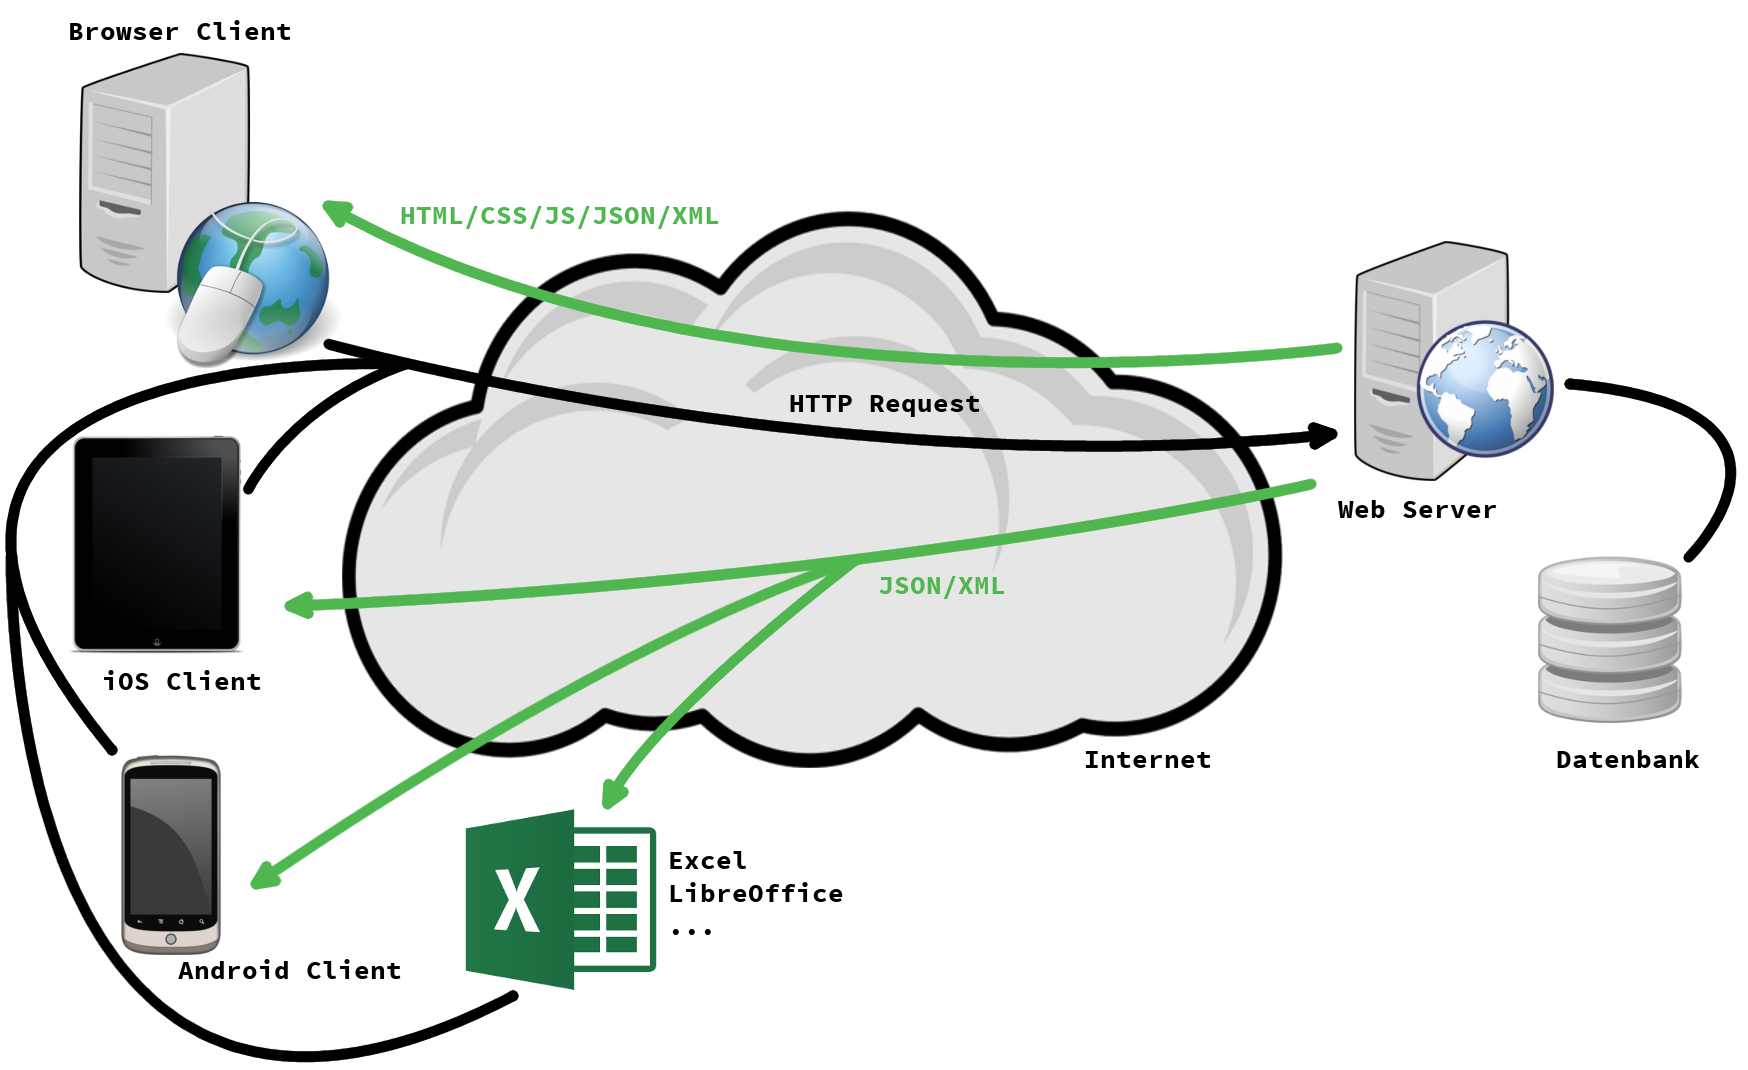
\includegraphics[width=0.6\textwidth]{img/webservice.png}
	\captionsetup{format=hang}
	\caption{Prinzip eines Webservice}
	\small Quelle: \url{https://www.ransoft.at/images/others/webservice.png}
	\label{fig:webservice}
\end{figure}
\section{Representational State Transfer (REST)}
\label{sec:rest}

\subsection{Funktionsweise einer \acs{REST}-Schnittstelle}
Um die Dreischichtenarchitektur zu etablieren, wird für den Datenaustausch zwischen Server--Front-End und Server--Datenbank auf das \acf{REST} gesetzt.
\acs{REST} ist ein Architekturstil für den Entwurf verteilter Netz"-werk"-an"-wen"-dung"-en.
Es setzt auf \acs{HTTP} und \acs{HTTPS}-Methoden und stellt verschiedene Methoden zur Verfügung.
Für den Einsatz von \acs{REST}-Services kommen folgende \acs{CRUD}-Prinzipien in Frage:

\begin{table}[ht]
	\renewcommand{\arraystretch}{1.2}
	\centering
	\begin{tabular}{l|l|l}
		\acs{CRUD} & \acs{HTTP} & Beispiel-\acs{URI} \\
		\hline
		Create & POST & http://lolcalhost:8080/cinema-system/movie \\
		Read & GET & http://lolcalhost:8080/cinema-system/show/1 \\
		Update & PUT & http://lolcalhost:8080/cinema-system/movie/5 \\
		Delete & DELETE & http://lolcalhost:8080/cinema-system/customer/4711 \\
	\end{tabular}
	\caption{\acs{CRUD}-Befehle und deren Verwendung}
	\label{tab:crud}
\end{table}

Wir die \acs{REST}-Schnittstelle mit einem \textit{POST} aufgerufen wird ein neuer Datensatz in der Datenbank angelegt.
In dem Beispiel aus Tabelle \vref{tab:crud} wird ein neuer Film in der Datenbank angelegt.
Die benötigten Informationen des Films werden über einen Form-Parameter (\textit{@FormParam}) im \acs{JSON}-Format an die \acs{REST}-Schnittstelle übertragen. %TODO Beispiel bringen
Wird in der Ressource die Schnittstelle mit einem \textit{GET} aufgerufen, wird ein Datensatz angefragt, der über einen anderen Webservice die Anforderung an die Datenbank sendet und anschließend wieder an die Ressource zurücksendet.
In dem Beispiel aus Tabelle \vref{tab:crud} wird die Ressource Film aufgerufen und der Datenbankeintrag mit der Film-ID 1 abgefragt.
Mittels \textit{PUT} wird ein vorhandener Datensatz aktualisiert.
In dem Beispiel aus Tabelle \vref{tab:crud} würde z.B. ein neuer Schauspieler hinzugefügt werden.
Schlussendlich löscht man einen Datensatz, indem man in der Ressource die Schnittelle mit \textit{DELETE} aufruft.
In dem Beispiel aus Tabelle \vref{tab:crud} würde man den Kunden mit der Kundennummer 4711 aus der Datenbank entfernen.\\

Während Anfragen über die \acs{REST}-Schnittstelle über den Server beantwortet werden, können auch verschiedene \acs{HTTP} bzw. \acs{HTTPS}-Status zurückgeliefert werden (siehe Tabelle \vref{tab:http_status}).

\begin{table}[!hpt]
	\renewcommand{\arraystretch}{1.2}
	\centering
	\begin{tabular}{l|p{8.5cm}}
		Status Code & Beschreibung \\
		\hline
		200 (OK) & Alles OK bei der Verbindung \\
		400 (Bad Request) & Der Server weiß nicht, was er mit der Anfrage machen soll \\
		401 (Unauthorized) & Der Client muss sich erst authentifizieren, z.B. falsches Passwort gewählt \\
		501 (Media Type unsupported) & Der gewählte Medientyp wird nicht unterstützt z.B. Text Plain oder es wird ein anderes Format erwartet z.B. \acs{JSON} \\
		503 (Service Unavailable) & Anfrage konnte nicht abgeschlossen werden
	\end{tabular}
	\caption{Mögliche \acs{HTTP}-Status eines Webservices}
\label{tab:http_status}
\end{table}
\clearpage

\subsection{Annotationen für eine \acs{REST}-Schnittstelle}
\label{ssec:annotationen_schnittstelle}

Das Paket JAX-RS von Jersey bietet eine Vielzahl an Möglichkeiten für Annotationen einer \acs{REST}-Schnittstelle.
In diesem Kapitel sollen einige im Projekt verwendete vorgestellt werden.

\subsubsection*{@Path}
Mittels \textit{@Path} werden die jeweiligen Pfade zu den \acs{REST}-Schnittstellen in einer Ressource dargestellt.
Diese können nach belieben geschachtelt werden.

So ist es z.B. möglich auf dem Server den Pfad zur Ressource der Reservierung anzugeben \textit{@Path("reservation")}.
Hier werden dann noch weitere Pfade wie \textit{@Path("book")} angegeben, der ausschließlich für das Buchen von Tickets oder \textit{@Path("block")}, der ausschließlich für das Blocken von Sitzen verantwortlich ist.
In ihnen sind dann verschiedenen \acs{CRUD}-Befehle definiert (vgl.~\nameref{sss:get}, \nameref{sss:post}, \nameref{sss:delete} auf Seite~\pageref{sss:delete}) 

\subsubsection*{@MediaType}
\label{sss:mediatype}
Die in diesem Projekt verwendete Annotation \textit{@MediaType} deklariert in jeder Ressource, welche Austauschformate zulässig sind. \\
Deklariert sind in diesem Projekt: \textit{MediaType.TEXT\_PLAIN\_TYPE}, sodass über das Front-End eine ID mitgegeben werden kann; \textit{MediaType.APPLICATION\_JSON\_TYPE}, sodass sichergestellt ist, dass nur ein \acs{JSON} als Austauschformat zulässig ist.

\subsubsection*{@Consumes}
\label{sss:consumes}
Mit Hilfe der Annotation \textit{@Consumes} definiert man an der \acs{REST}-Schnittstelle, dass eine Verarbeitung nur mit dem gewünschten MediaType erfolgt.
Wird dies nicht erfüllt, kommt die Fehlermeldung 501 (vgl. Tabelle \vref{tab:http_status}).

\subsubsection*{@FormParam}
\label{sss:formparam}
Über die Annotation \textit{@FormParam} wird in der \acs{REST}-Schnittstelle festgelegt, dass das \acs{JSON} aus dem Front-End ein bestimmter String vor dem eigentlichen \acs{JSON} erwartet wird. \\
Ein korrektes \acs{JSON} mit \textit{@FormParam} für das Blocken würde z.B. folgendermaßen aussehen: \textit{block=\{ <DATEN> \}}
\subsubsection*{@GET}
\label{sss:get}
Über die \textit{@GET}-Annotation wird eine einfache Anfrage erstellt.
So ist sichergestellt, dass auch nur die \acs{REST}-Schnittstelle aufgerufen wird, die die \textit{@GET}-Annotation hat, obwohl es vielleicht nochmals die selbe Methode gibt für einen POST.

\subsubsection*{@POST}
\label{sss:post}
Über die \textit{@POST}-Annotation wird sichergestellt, dass wirklich das übergebene \acs{JSON} in die in diesem Projekt verwendete Datenbank gespeichert werden soll.

\subsubsection*{@DELETE}
\label{sss:delete}
Über die \textit{@DELETE}-Annotation wird sichergestellt, dass wirklich der übergebene \textit{String} z.B. eine ID in der in diesem Projekt verwendeten Datenbank gelöscht werden soll.

\subsubsection*{@Produces}
\label{sss:produces}
Über die Annotation  \textit{@Produces} wird an der \acs{REST}-Schnittstelle definiert, dass ausschließlich die deklarierten Medien-Typen wie z.B. TEXT\_PLAIN oder JSON erzeugt werden (vgl. \nameref{sss:mediatype}).
\section{JavaScript Object Notation (JSON)}
\label{sec:json}
Für den Datenaustausch zwischen Front- und Backend wird mittels der \ac{JSON} realisiert. Grund ist, dass hier rein die Nutzdaten transferiert werden. Ferner gestalte sich das Auslesen und Generieren der \ac{JSON}-Dateien als recht \enquote{einfach}. \\
Ein Array bzw. Liste wird in \ac{JSON} mit [ ] dargestellt. Objekte werden mit \{ \} dargestellt. Jedes Attribut und jede Zeichenkette wird in \ac{JSON} in Anführungszeichen gesetzt (siehe Quelltext \vref{lst:example_movie}).  

\begin{minipage}{\linewidth}
\begin{lstlisting}[language=json,firstnumber=1]
{"movie": {
	"id": 1,
	"title": "Kampf der Titanen",
	"duration": 120,
	"hall":
	{
	"id": 1,
	"name": "Kino 1,
	"seats": [{"seat":{"id":1, ...}}]
	}, 
	"shows": [{"show":{"id":1, ...}}]
	}
}
\end{lstlisting}
\captionof{lstlisting}{Beispiel eines Films im JSON-Format}
\label{lst:example_movie}
\end{minipage}
\section{Generieren der \acf{JSON}}
\label{sec:json_generieren}
\authorsection{\authorSG}

Java ist eine objektorientierte Sprache.
Alle Klassen sind dementsprechend als Objekte hinterlegt.
Durch die Implementierung eines sog. Object-Mappers wie dem Jackson-Mapper\footnote{\url{https://github.com/FasterXML/jackson}}
ist es möglich die zuvor erstellten Objekte in eine \acs{JSON}-Datei zu überführen.
Er erkennt automatisch, ob es sich um ein Objekt, ein Attribut oder eine Liste handelt.
Der Programmierer ruft lediglich die Methode writeValueAsString(Object-to-JSON) auf. \\
Das Auslesen eines \acs{JSON}-Strings wird mittels der Methode readValue(json, javaClass) ausgeführt.
Der Vorteil dieser Methode ist, dass hier die Java-Klasse angegeben wird, also das Objekt, in das der \acs{JSON}-String konvertiert werden soll.

Der Jackson-Mapper wird in diesem Projekt über eine Dependency zu einem Maven-Projekt hinzugefügt und kann anschließend verwendet werden (siehe Quelltext \ref{lst:Einbindung_ObjektMapper}) %TODO VARIOREF

\begin{minipage}{\linewidth}
\begin{lstlisting}[language=XML]
<dependency>
	<groupId>com.fasterxml.jackson.core</groupId>
	<artifactId>jackson-databind</artifactId>
	<version>2.9.4</version>
</dependency>
\end{lstlisting}
\captionof{lstlisting}{Einbindung des Objekt-Mappers in die pom.xml}
\label{lst:Einbindung_ObjektMapper}
\end{minipage}

\begin{minipage}{\linewidth}
	\begin{lstlisting}[style=lstJava]
	public static String toJSON ( Object object ) throws JsonProcessingException
	{
		String str = "";
		ObjectMapper om = new ObjectMapper();
		om.getSerializerProvider().setNullKeySerializer(nullKeySerializer);
		str = om.writeValueAsString(object);
		return str;
	}
	
	public static Object fromJSON ( String json, Class<?> javaClass ) throws IOException
	{
		ObjectMapper om = new ObjectMapper();
		om.configure(DeserializationFeature.FAIL_ON_UNKNOWN_PROPERTIES, false);
		Object obj = om.readValue(json, javaClass);
		return obj;
	}
	\end{lstlisting}
	\captionof{lstlisting}{Ausschnitt aus der selbst erstellten Klasse JSONConverter}
\end{minipage}
% !TEX root =  master.tex
\section{\acf{DTO}}
\label{sec:dto}
Das \ac{DTO} ist ein Entwurfsmuster aus dem Bereich der Softwareentwicklung.
Es wird genutzt, um mehrere Objekte in einem Programmaufruf zusammenzufassen, weshalb es Anwendung in verteilten Systemen findet.

Ein \ac{DTO} entspricht eigentlich dem \ac{POJO}.
Es hat nahezu die selben Attribute, kann aber nach Belieben verändert werden.
So kann man sich mittels des \ac{DTO} nur einige Attribute anzeigen lassen und die Entität bleibt unberührt.

Die \acsp{DTO} werden in diesem Projekt dazu genutzt, um die Daten aus der Datenhaltungsschicht der Drei-Schichten-Architektur in die Logik- bzw. Fachkonzeptschicht zu transferieren. Denn eine Entität verlässt niemals die Datenhaltungsschicht.
Von dort aus werden sie an die Benutzerschicht weitergeleitet.

\subsection{Umwandlung der Entität zu und von einem \acf{DTO}}
\label{ssec:umwandlung_dto}
Wie bereits beschrieben kommen in diesem Projekt \acp{DTO} zum Einsatz. Um eine Umwandlung zu realisieren wurden zwei Java-Klassen implementiert: \textit{EntityToToHelper} und \textit{ToToEntityHelper}. \\

Die Klasse \textit{EntityToToHelper} ist dafür verantwortlich, die zuvor über das \acs{DAO} angefragte Entität mit all ihren Attributen in ein \acs{DTO} umzuwandeln, sodass es transferierbar ist. \\
Ein Beispiel für die Umwandlung in ein \acs{DTO} befindet sich im Anhang \vref{lst:EntityToToHelper_movie}. \\
Die Klasse \textit{ToToEntityHelper} ist dafür verantwortlich die zuvor über das \acs{JSON} übermittelte \acs{DTO} mit all seinen Attributen in ein Entität umzuwandeln, sodass es persistier-, änder- oder löschbar ist.\\ 
Ein Beispiel für die Umwandlung in eine Entität befindet sich im Anhang \vref{lst:ToToEntityHelper_movie}.

% !TEX root =  master.tex
\section{Sitzplatzauswahl und Blockierungen}
\authorsection{\authorNL}

Beim Reservierungsvorgang ist es essentiell, dass ein Sitzplatz nicht mehrfach reserviert wird.

Hier ein einfaches Beispiel:
Benutzer A besucht die Seite, wählt einen Film und eine Vorstellung aus.
Die Saalübersicht wird geladen, wobei Sitzplätze, die bereits reserviert sind, optisch hervorgehoben sind und nicht mehr ausgewählt werden können.
Etwa zur gleichen Zeit besucht Benutzer B die Seite.
Er wählt die selbe Vorstellung, sieht die gleiche Saalübersicht und wählt einen Platz aus: Reihe 4, Platz 2.
Benutzer B folgt daraufhin den weiteren Schritten, bezahlt seinen Sitzplatz und erhält eine Bestätigung, dass Reihe 4, Platz 2 erfolgreich von ihm gebucht wurde.
Auch Benutzer A hat Reihe 4, Platz 2 ausgewählt.
Zu dem Zeitpunkt als Benutzer A den Saalplan geladen hat, war die Reservierung von Benutzer B noch nicht abgeschlossen, sodass der Platz frei war.
Auch Benutzer A möchte nun das Ticket bezahlen, muss aber eine Fehlermeldung erhalten, damit das Ticket für Reihe 4, Platz 2 nicht doppelt verkauft wird.

Spätestens bei der verbindlichen Reservierung und der normalerweise folgenden Bestätigung muss eine Fehlermeldung erscheinen, wenn der Platz bereits belegt ist.
Im Idealfall wird der Nutzer aber schon früher benachrichtigt, wenn er einen Platz ausgewählt hat, der in der Zwischenzeit von einem anderen Benutzer reserviert wurde.

Der Fall, dass ein Platz durch einen anderen Benutzer reserviert wird, ist mit gewisser Wahrscheinlichkeit vorhersehbar.
Wählt ein Benutzer im Saalplan ein paar Plätze aus, so wird er vermutlich in den nächsten paar Minuten mit der Bezahlung fortfahren und die Plätze für sich reservieren.
In dem Moment, wo ein Benutzer einen Sitzplatz also nur auswählt, kann diese Information bereits in der Datenbank gespeichert werden.
Der Sitzplatz wird für diesen Benutzer zwar nicht reserviert, aber für einen kurzen Zeitraum vorgemerkt.
Will nun jemand einen Platz auf dem Saalplan auswählen, teilt er dies über die \acs{API} dem Back-End mit.
Nun gibt es mehrere mögliche Ergebnisse:
\begin{enumerate}
\item Der ausgewählte Sitzplatz ist bereits reserviert.
\item Der ausgewählte Sitzplatz ist bereits für einen anderen Benutzer vorgemerkt, könnte also in einigen Minuten wieder frei werden.
\item Der Sitzplatz ist weder reserviert, noch vorgemerkt.
Er wurde nun erfolgreich für den aktuellen Benutzer vorgemerkt.
\end{enumerate}

Dies kann nun dazu führen, dass ein Benutzer einen freien Saalplan angezeigt bekommt und beim Anklicken eines Platzes dieser nun nicht mehr als \enquote{frei}, sondern als \enquote{durch einen anderen Nutzer belegt} angezeigt wird.

Die zu der Reservierung zugehörigen Operationen auf der Datenbank müssen atomar ausgeführt werden, sodass die Reservierung entweder erfolgreich war oder eine Fehlermeldung den Benutzer informiert, dass die Reservierung fehlgeschlagen ist.

Alle Sicherheitsprüfungen müssen im Back-End ausgeführt werden.
Natürlich können auch einzelne Prüfungen im Front-End implementiert werden, diese helfen allerdings nur einem normalen Benutzer den Vorgang zu erleichtern.
Eine Absicherung bieten derartige Prüfung im Front-End nicht, da der clientseitig ausgeführte Quellcode logischerweise vom Client verändert werden kann und jeder Angreifer eine manipulierte Anfrage mit selbst gewählten Parametern an die \acs{API} schicken kann.
\section{Reservieren}
\label{sec:reservieren}

\subsection{Herausforderung}
\label{ssec:herausforderung_reservieren}

Eine weitere Herausforderung bestand darin, das Reservieren eines Sitzes im Back-End zu realisieren.
Hierfür mussten ebenso verschiedene Aspekte betrachtet werden.

\begin{enumerate}
	\label{enum:reservieren}
	\item \label{itm:zeitpunkt_reservieren}Das Reservieren darf nur, wie das Blocken, bis zu einem bestimmten Zeitpunkt möglich sein.
	\item \label{itm:geblockt_durch_benutzer} Falls der Sitzplatz durch den selben Benutzer geblockt wurde, darf dieser diesen buchen.
	Andernfalls darf es keine erfolgreiche Reservierung geben.
	\item \label{itm:mehr_eine_vorstellung_reservieren}Eine Mehrfachvergabe des selben Sitzplatzes für eine Vorstellung muss wie beim Blocken ausgeschlossen sein (vgl. Herausforderung \ref{enum:blocken} Punkt \ref{itm:mehr_eine_vorstellung}).
	\item \label{itm:mehr_mehrere_vorstellungen_reservieren}Die Belegung eines Sitzes für verschiedene Vorstellungen muss gewährleistet sein.
	\item \label{itm:ticket_reservieren} Der Sitzplatz darf nur reserviert werden, wenn es für ihn noch kein Ticket gibt und er derzeit auch nicht blockiert ist.
	\item \label{itm:front_end_reservieren} Eine Information mit den erfolgreich reservierten Sitzen muss an das Front-End gesendet werden.
	\item \label{itm:zeit_reservieren} Der Zeitpunkt der Reservierung darf durch das Front-End nicht manipulierbar sein.
\end{enumerate}

\subsection{Lösungsansatz}
\label{ssec:loesung_reservieren}

Um die geforderten o.g. Punkte umzusetzen, werden in der \acs{REST}-Schnittstelle \\\jinline |reservation/book| mehrere Überprüfungen durchgeführt.

\subsubsection*{Punkt \ref{itm:zeitpunkt_reservieren} -- Zeitpunkt}
\label{ssssec:Zeitpunkt_reservieren}
Siehe \nameref{ssec:loesung_blocken} \nameref{ssssec:Zeitpunkt} auf Seite \pageref{ssssec:Zeitpunkt}.

\subsubsection*{Punkt \ref{itm:geblockt_durch_benutzer} -- Geblockt durch Benutzer, Punkt \ref{itm:mehr_eine_vorstellung_reservieren}, \ref{itm:mehr_mehrere_vorstellungen_reservieren} -- Mehrfachvergabe, Punkt \ref{itm:ticket_reservieren} -- Reservieren}
\label{ssssec:geblockt_durch_benutzer}
Um einem Benutzer das Reservieren des möglicherweise geblockten Sitzplatzes für eine Vorstellung zu gewährleisten, wurde, wie bereits erwähnt, sich dazu entschlossen einen Sessiontoken als Identifikator mitzugeben.
Da dieser vom Front-End erzeugt wird, reicht dieses den Sessiontoken beim Reservierungsvorgang im \acs{JSON} mit.
Da der Sessiontoken auch hier nach erfolgreicher Buchung nicht übermittelt werden soll, gibt es auch für diesen Anwendungsfall zwei \acp{DTO}, die wie im \nameref{ssec:loesung_blocken} Blocken in \nameref{ssssec:Bezeichner} auf Seite \pageref{ssssec:Bezeichner} auch die \acs{JSON}-Annotation, für das Schreiben bzw. Nichtschreiben des Sessiontokens, besitzen (\textit{BookingToWithSessiontoken} und \textit{BookingTo}). 

Auch hier erfolgt durch eine ausgelagerte Methode \jinline |checkIfSeatsAreBookable| die Überprüfung, ob
\begin{enumerate}
	\item es bereits ein Ticket für den zu buchenden Sitzplatz gibt.
	\item der Sitzplatz bereits geblockt ist.
	\begin{enumerate}
		\item Wenn ja, passt der Sessiontoken der aktuellen Anfrage zu diesem? Dann darf die Buchung erfolgen.
		\item Falls nicht, darf die Reservierung nicht erfolgen.
	\end{enumerate}
\end{enumerate}

War dieser Methoden-Aufruf erfolgreich, wird eine weitere Methode aufgerufen, die ein Reservierungs-\acs{DTO} als Rückgabewert hat (\jinline |createReservationForSeats|). \\
Dieses ist mit dem aktuellen Datum und der aktuellen Uhrzeit sowie einer Liste mit Ticket-\acp{DTO} versehen.
Dem Ticket-\acs{DTO} wird der aktuelle Sitzplatz zugeteilt.
Ferner wird in jedem Ticket-\acs{DTO} individuell das Attribut \jinline |isReducedPrice| gesetzt, welches zuvor durch das Front-End zu dem jeweiligen Sitzplatz über das \acs{JSON} mitgeteilt wurde.
Durch dieses Setzen des Attributs hat man im Nachhinein die Möglichkeit, die korrekte Preisberechnung zu verifizieren.

Die Implementierung, ob die ausgewählten Sitzplätze verfügbar sind, befindet sich im Anhang \vref{lst:Angang_Prüfung_ob_Reservierung_möglich}.
Die Implementierung für das Erstellen des Reservierungs-\acp{DTO} befindet sich im Anhang \vref{lst:Anhang_Erstellen_Reservierung}.

\subsubsection*{Punkt \ref{itm:front_end_reservieren} -- Erfolgreich}
\label{ssssec:front_end_reservieren}
Wurde der Reservierungsvorgang erfolgreich durchgeführt, erhält das Front-End das Reservierungs-\acs{DTO} als \acs{JSON} wie in \nameref{ssec:loesung_blocken} im \nameref{ssssec:erfolgreich_blocken} auf Seite \pageref{ssssec:erfolgreich_blocken} beschrieben, zur Auswertung zurück (vgl. Herausforderungen Punkt \vref{itm:front_end_reservieren}).
Diese wertet das \acs{JSON} aus und generiert daraus einen \acs{QR-Code}, der im Browser angezeigt wird.
Ein Beispiel für die Umsetzung seitens des Front-Ends befindet sich in Kapitel \vref{fig:vorstellung04}.
%Dieses hat wie zuvor beschrieben das Attribut \jinline |sessiontoken| nicht gesetzt.


% !TEX root =  master.tex
\chapter{Front-End}

\section{Technologien}
\label{sec:technologien}

Für das hier erstellte Kinoreservierungsprogramm wurde die Verwendung von Java\footnote{\url{https://java.com/de/download/} -- Version 8.0.141 verwendet} für das Back-End vorgegeben. 

Als Java-\acs{IDE} kommt Eclipse\footnote{\url{https://www.eclipse.org/} -- Version: Photon Release (4.8.0)} zum Einsatz, da es aus vorangegangenen Vorlesungen bekannt ist.
Für die Kommunikation zwischen den einzelnen Schichten der Drei-Schichten-Architektur kommen \acs{REST}ful-Webservices in Verbindung mit Jersey\footnote{\url{https://jersey.github.io/} -- Version 1.19.4} sowie \acp{DTO} zum Einsatz (Kapitel \vref{sec:dto}), die zwischen den einzelnen Schichten transferiert werden.

Um eine Datenhaltung und den Austausch von Informationen zu gewährleisten, wurde sich in dieser Arbeit für eine Postgres Datenbank entschieden.
Der Zugriff auf die Datenbank erfolgt mittels der \ac{JPA} in Verbindung mit EclipseLink (Kapitel \vref{ssec:jpa}).
% !TEX root =  master.tex
\section{Startseite mit Filmübersicht}

Auf der Startseite sieht der Benutzer direkt das Kinoprogramm.
Ganz oben befindet sich ein \enquote{Karussell} mit den aktuellen Blockbustern.
Direkt darunter folgt dann die Liste mit den Filmen.

\begin{figure}[ht]
	\centering
	\subfloat[Desktop-Computer]{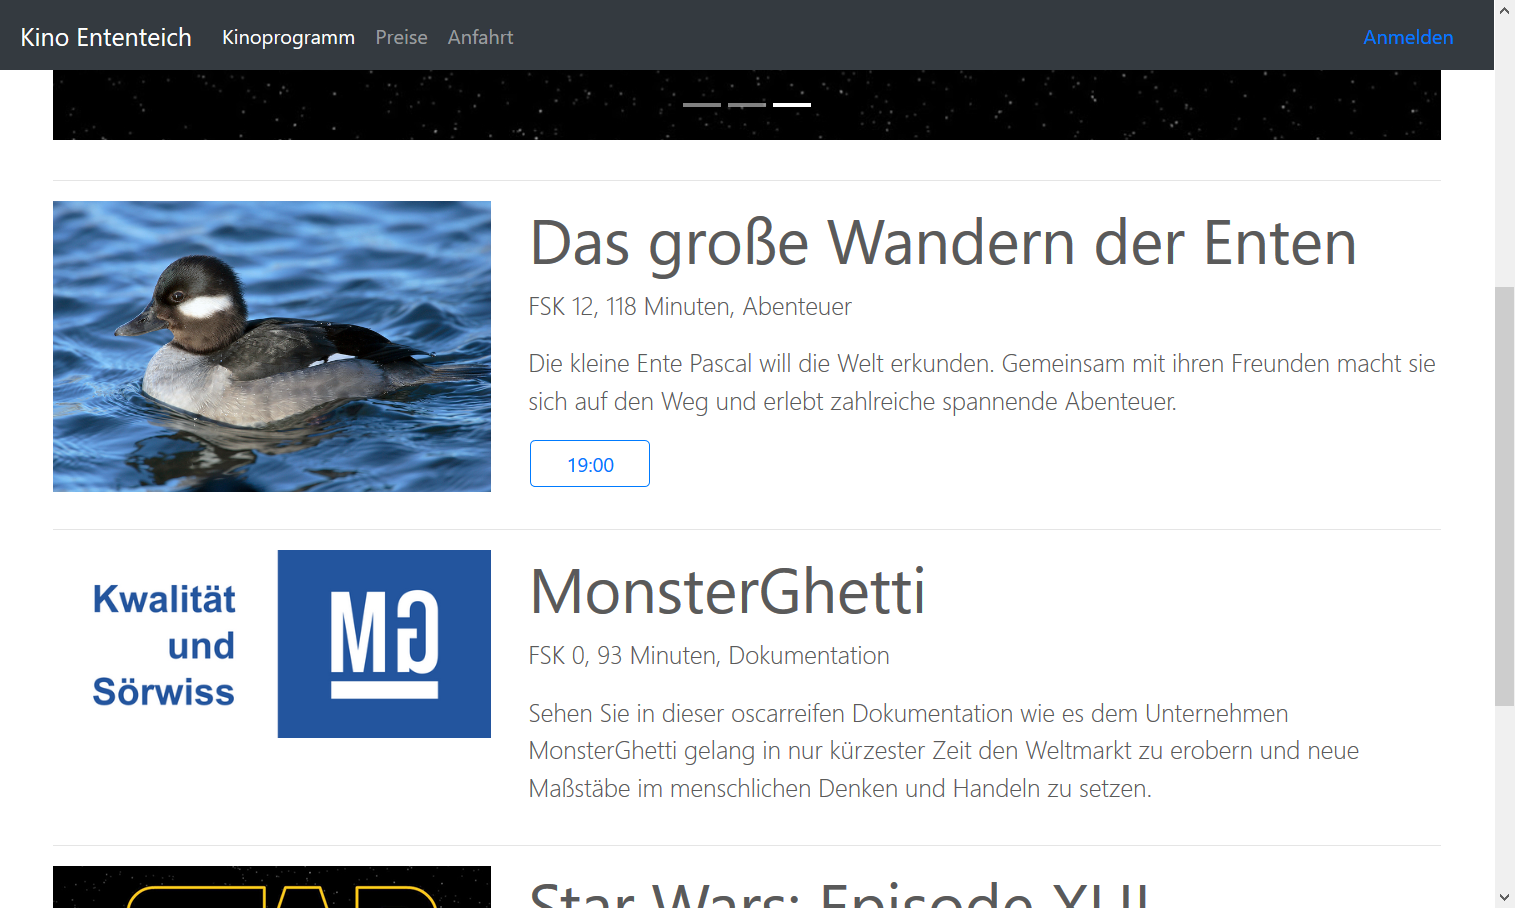
\includegraphics[height=0.28\textheight]{img/screenshots/startseite01}
	\label{fig:startseite01}}
	\hfill
	\subfloat[Mobiles Gerät]{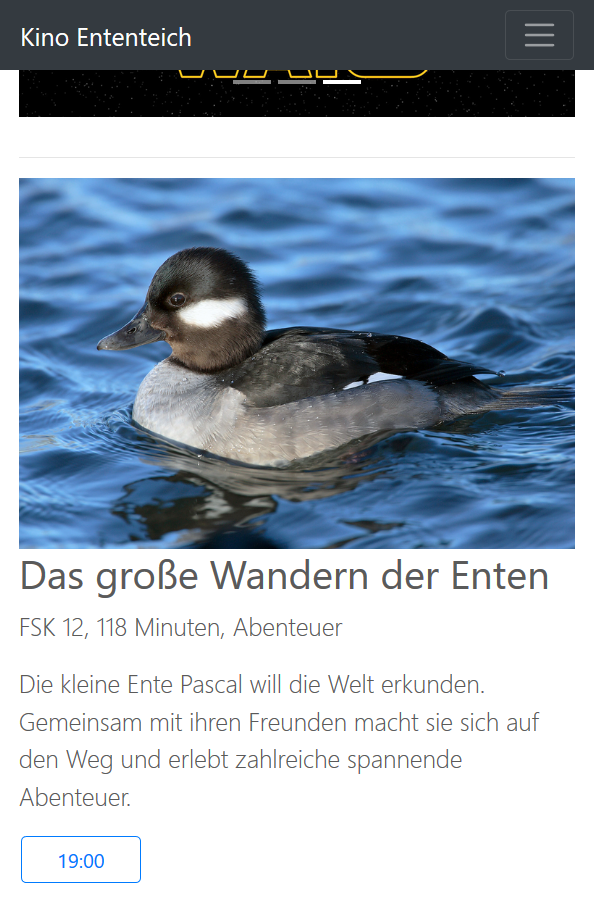
\includegraphics[height=0.28\textheight]{img/screenshots/startseite02}
	\label{fig:startseite02}}
	\caption{Filmübersicht auf der Startseite}
\end{figure}

Dabei ist zu jedem Film neben dem Titel auch noch ein Bild zu sehen.
Allgemeine Informationen zum Film sowie eine Beschreibung ermöglichen es dem Benutzer, sich einen schnellen ersten Eindruck von dem jeweiligen Film zu verschaffen.
Durch Anklicken des Filmtitels oder des Bildes gelangt man zu den Vorstellungen und weiteren Details.
Um Benutzern einen Klick zu ersparen, sieht man sogar direkt die heutigen Vorstellungen und kann gegebenenfalls sofort zu diesen Vorstellungen springen und Sitzplätze auswählen.

Je nach Größe des Bildschirms, wir der Inhalt entsprechend angezeigt.
Bei breiten Bildschirmen, wie es meist bei Desktop-Computern und Laptops der Fall ist, ist genügend Platz, um Bild und Text nebeneinander anzuzeigen.
Bei Smartphones hingegen, wäre das Bild so kaum erkennbar und es würden nicht viele Wörter in eine Zeile passen.
Dementsprechend werden bei solchen Bildschirmen Bild und Text untereinander angezeigt.
All diese Anpassungen werden durch \acs{CSS}-Anweisungen veranlasst, inhaltlich gibt es keine Unterschiede.
% !TEX root =  master.tex
\section{Anbindung an das Back-End}
\label{sec:anbindung_backend}

Um die Daten aus der Datenbank bzw. dem Back-End anzuzeigen, werden diese durch einen oder mehrere \acs{AJAX}-Aufrufe nachgeladen.
Beim Laden der Startseite wird die Funktion \textit{loadMovies()} aufgerufen.
Diese wiederum ist nur für die Zuordnung von einem Pfad bzw. einer \acs{URI} zu einer Funktion, die das Ergebnis verarbeitet, da.
Sie würde auch \acs{URL}-Parameter auslesen und in den Aufruf mit einarbeiten, dies ist aber auf der Startseite noch nicht notwendig.

\begin{lstlisting}[language=JavaScript]
const URL_SERVER = "http://localhost:8080/cinema-system";
const PATH_ALL_MOVIES = "/movie/getAllMovies";

function getData (path, func) {
	$.ajax({
		type: "GET",
		url: URL_SERVER + path,
		success: (data) => func(data),
		error: function (xhr,status,error){
			console.log(xhr, status, error);
			func([]);
		}
	});
}

function loadMovies () {
	getData(PATH_ALL_MOVIES, displayMovies);
}

function displayMovies (movies) {
	...
}
\end{lstlisting}
\captionof{lstlisting}{\acs{AJAX}-Aufruf, um alle Filme zu erhalten}
\label{lst:ajax_all_movies}
% !TEX root =  master.tex
\section{Filmdetails und Vorstellungsauswahl}

Nachdem die Daten wie in Quelltext \ref{lst:load_movie_and_shows} geladen wurden, muss nun das \acs{DOM} entsprechend verändert werden.
Die statische \acs{HTML}-Seite ist dabei auf das Wesentliche reduziert und enthält neben der Menüleiste und der Fußzeile folgenden Teil:

\begin{lstlisting}[style=lstHTML]
<div class="container" id="movie">
	<!-- Informationen zum Film werden hier eingefügt -->
	<table class="table" id="shows">
		<tr>
			<th>Tag</th>
			<th>Vorführungen</th>
		</tr>
		<!-- die einzelnen Vorstellungen werden hier eingefügt -->
	</table>
	<!-- Bewertungen werden hier eingefügt -->
</div>
\end{lstlisting}
\captionof{lstlisting}{\acs{HTML}-Seite für Filmdetails}
\label{lst:html_movie_and_shows}

An den gekennzeichneten Stellen wird später der Inhalt, der aus dem Back-End geladen wurde, eingefügt.
Dafür gibt es kleinere Vorlagen mit Platzhaltern.
In Quelltext \ref{lst:html_template_movie_detail} sieht man die Vorlage für die Filmdetails.

\begin{lstlisting}[style=lstHTML,escapeinside=``]
<div class="row featurette">
	<div class="col-12 col-sm-4">
		<img class="featurette-image img-fluid mx-auto" src="./img/`\textcolor{red}{\{movieID\}}`.jpg" alt="`\textcolor{red}{\{movieTitle\}}`" width="100%">
	</div>
	<div class="col-12 col-sm-8">
		<h2 class="featurette-heading">`\textcolor{red}{\{movieTitle\}}`</h2>
		<p class="lead">FSK `\textcolor{red}{\{movieFSK\}}`, `\textcolor{red}{\{movieDuration\}}` Minuten, `\textcolor{red}{\{movieGenres\}}`</p>
		<p class="lead rating-`\textcolor{red}{\{movieRatingRounded\}}`">`\textcolor{red}{\{movieRating\}}`</p>
	</div>
</div>

<div class="row featurette">
	<div class="col-12">
		<p class="lead">`\textcolor{red}{\{movieDescription\}}`</p>
	</div>
</div>
\end{lstlisting}
\captionof{lstlisting}{\acs{HTML}-Vorlage mit Platzhaltern für Filmdetails}
\label{lst:html_template_movie_detail}

In JavaScript wird diese Vorlage dann mit Inhalten befüllt.
Nachdem die Daten in der Funktion \textit{displayMovieAndShows()} ein wenig verarbeitet wurden, können sie mit JavaScript bzw. jQuery in die Vorlage und danach ins \acs{DOM} eingefügt werden.

\begin{lstlisting}[language=JavaScript]
$("#movie").prepend(templateMovieDetail
	.replace("{movieID}", movie.id)
	.replace(/\{movieTitle\}/g, movie.name)
	.replace("{movieFSK}", movie.fsk)
	.replace("{movieDuration}", movie.duration)
	.replace("{movieGenres}", genres)
	.replace("{movieRatingRounded}", Math.max(0, Math.min(5, Math.round(rating))))
	.replace("{movieRating}", (movie.ratings.length > 0 ? rating.toFixed(1).replace(".",",") : "") + " (" + movie.ratings.length + " Bewertung" + (movie.ratings.length == 1 ? "" : "en") + ")")
	.replace("{movieDescription}", movie.description)
);
\end{lstlisting}
\captionof{lstlisting}{Einfügen der Filmdetails ins \acs{DOM} mit jQuery}
\label{lst:js_write_movie_detail_to_dom}

Genauso wie die Filmdetails werden auch die Vorstellungen und die Bewertungen ins \acs{DOM} eingefügt.

Zusammenfassend heißt das, dass zuerst einmal die statische und weitestgehend leere \acs{HTML}-Seite geladen wird.
Diese wiederum importiert eine JavaScript-Datei, welche beim Laden der Seite einen Aufruf an das Back-End schickt.
Sobald der Server antwortet, wird die Antwort entsprechend verarbeitet und in JavaScript in kleinere Vorlagen eingefügt.
Die mit Inhalten befüllten Vorlagen werden dann mit jQuery ins \acs{DOM} eingefügt, sodass die \acs{HTML}-Seite die gewünschten Inhalte darstellt.
Dies passiert im Idealfall so schnell, dass es für den Benutzer wirkt, als hätte er die Seite \enquote{ganz normal} geladen.

Damit dies reibungslos funktioniert, ist es essentiell, dass sich die Kommunikation mit dem Server auf ein Minimum beschränkt und keine nicht benötigten oder redundanten Daten transferiert werden.
So ist es zum Beispiel schlecht für die Performance, wenn man im Front-End lediglich eine Liste mit allen Filmen sehen will, aber vom Back-End zu jedem Film alle Vorstellungen mit allen Sitzplätzen erhält.

Genauso muss natürlich die Verarbeitung im Front-End effizient erfolgen.
% !TEX root =  master.tex
\section{Implementierung des Saalplans}
\authorsection{\authorNL}

\subsection{Darstellung des Kinosaals}

Eine zentrale Aufgabe im Front-End war es, den Kinosaal mit den Sitzen anzuzeigen und dem Benutzer zu ermöglichen, Plätze auszuwählen.

Dies lässt sich mit einfachen Mitteln auch in \acs{HTML} umsetzen, z.B. mit \textit{div}-Elementen, bei denen man Größe und Farbe festlegt.
Mit JavaScript wird dann implementiert, was passiert wenn ein Sitzplatz angeklickt wird.

\begin{figure}[ht]
	\centering
	\subfloat{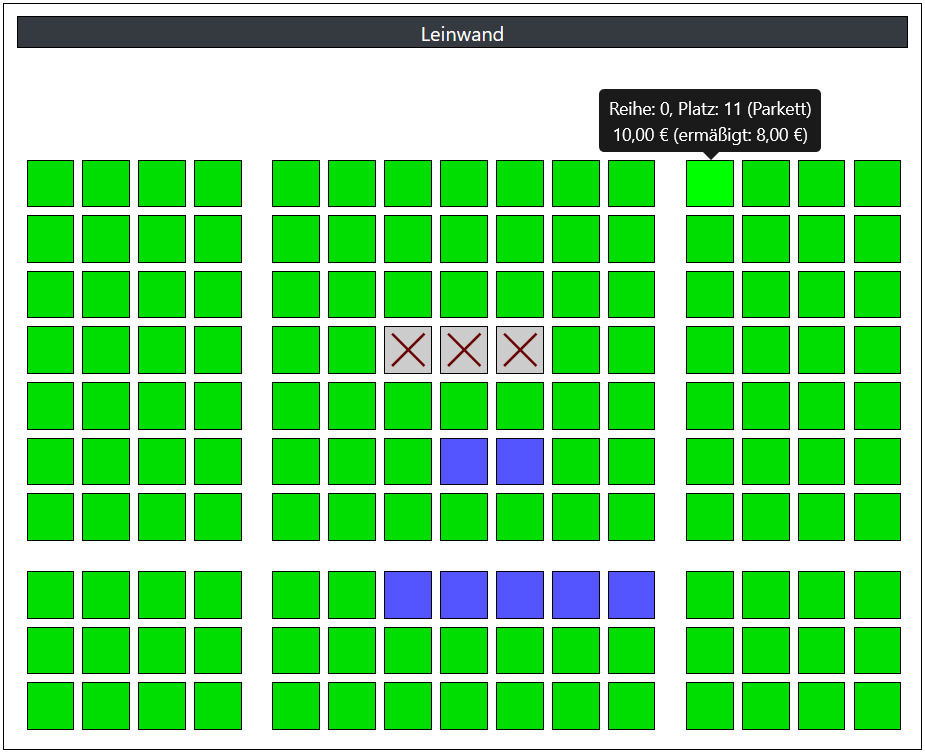
\includegraphics[height=0.295\textheight]{img/screenshots/saalplan01}}
	\hfill
	\subfloat{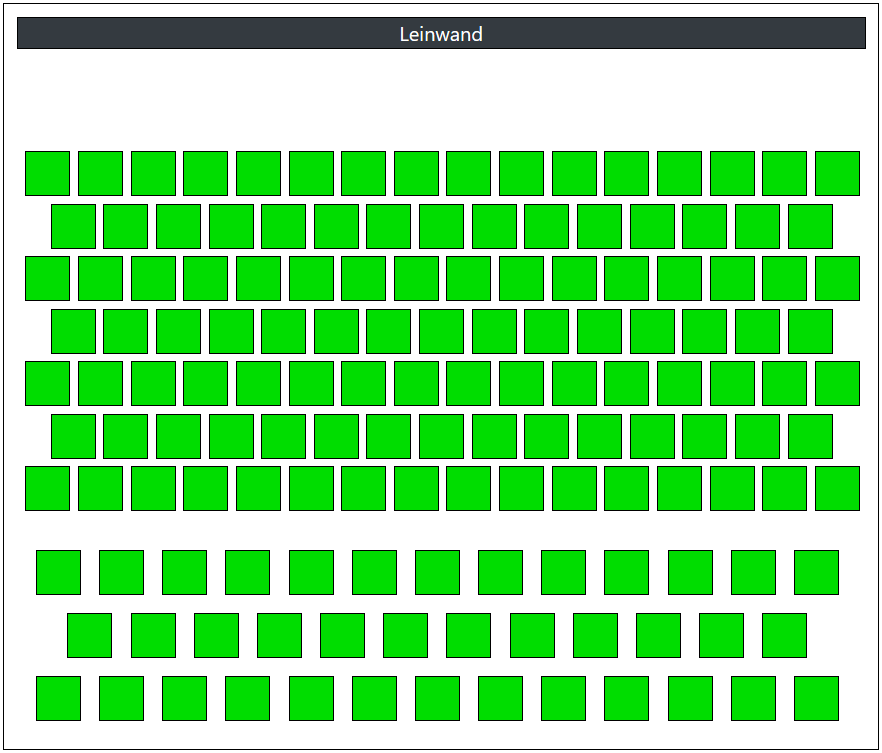
\includegraphics[height=0.295\textheight]{img/screenshots/saalplan03}}

	\caption{Saalpläne}
	\label{fig:saalplan}
\end{figure}

In Abbildung \vref{fig:saalplan} kann man sehen, wie der Kinosaal im Browser dargestellt wird.
Eine Box außen bildet die Umrandung und stellt den Saal dar.
Darin befindet sich eine zweite farblich hervorgehobene Box, die die Leinwand abbildet, damit die Benutzer wissen, wo im Kinosaal vorne und hinten ist, und sie somit ihre Entscheidung, wo sie sitzen möchten, treffen können.
Darunter finden sich dann die Sitzplätze.

Die Sitzplätze sind dabei farblich gekennzeichnet, um anzuzeigen, ob ein Sitzplatz frei oder belegt ist.
Belegte Sitze sind einerseits grau, andererseits auch noch mit einem Kreuz versehen, um Menschen, die in ihrer Farbwahrnehmung eingeschränkt sind, zu berücksichtigen.
Außerdem werden ausgewählte Sitze blau markiert und der Sitz, über dem aktuell die Maus ist, wird ebenso hervorgehoben.
Ein Tooltip mit einer kurzen Beschreibung und Details zu Kategorie und Preis, gibt dem Benutzer weitere Informationen.

Das Aussehen der Sitzplätze wird über Klassen und eine eigene \acs{CSS}-Datei definiert, sodass sich dies schnell anpassen lässt und zum Beispiel die Farbe der Sitzplätze mit einem Mal änderbar ist.

\begin{figure}[ht]
	\centering
	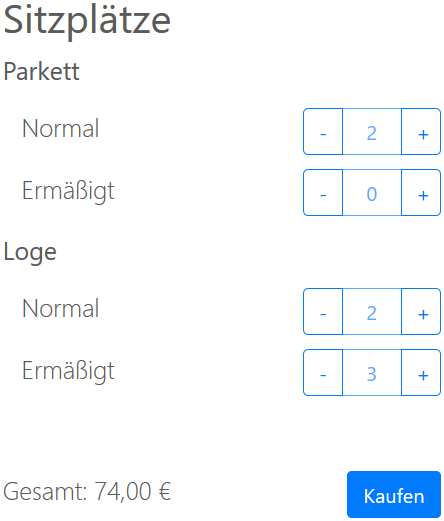
\includegraphics[width=0.4\textwidth]{img/screenshots/saalplan02}
	\captionsetup{format=hang}
	\caption{Preisstufen}
	\label{fig:saalplan02}
\end{figure}

Wählt man nun Sitzplätze aus, so muss man noch angeben, wie viele Tickets zum normalen Preis man kaufen möchte und wie viele zu einem ermäßigten Preis.
Daraus wird dann direkt der Preis berechnet und angezeigt (siehe Abbildung \ref{fig:saalplan02}).
Je nach Bildschirmgröße und -dimensionen werden diese Element neben dem Saalplan oder darunter angezeigt.
Mit dem \enquote{Kaufen}-Button gelangt man dann zur nächsten Seite, um weitere Daten anzugeben.

In der ersten Implementierung wurden der Saal und die Sitzplätze mit absoluten Größenangaben definiert.
So hatte das \textit{div}-Element, das einen Sitzplatz darstellt, als Höhe und Breite \textit{20px} gesetzt und eine Position relativ zur links oberen Ecke des Saals in Pixeln angegeben.
Die Koordinaten kommen dabei direkt aus dem Back-End bzw. der Datenbank.
Dies ermöglicht es, nicht nur einfach alle Plätze nebeneinander anzuzeigen, sondern auch Gänge einzufügen, Plätze versetzt anzuordnen, die Abstände zwischen den Sitzen individuell zu gestalten und somit den Saalplan an die Realität anzupassen.

Durch die Verwendung absoluter Größen in Pixeln, ist jedoch das Benutzererlebnis auf kleinen Bildschirmen schlechter.
Der Saal ist erst einmal breiter als der Bildschirm und der Benutzer muss herauszoomen und die Größe selbst anpassen.
Das Gleiche gilt für Benutzer eines Desktop-Computers, wenn sie die Fenstergröße anpassen.

Um dies zu verbessern, wird beim erstmaligen Laden sowie bei jeder Änderung der Fenstergröße, die Größe des Saals und der Sitzplätze neu berechnet.
Die Größenangaben aus der Datenbank werden dabei genutzt und entsprechend skaliert, sodass der Saalplan weder die volle Breite, noch die volle Höhe des Bildschirms überschreitet.
Um den Berechnungsaufwand zu reduzieren, sind die Koordinaten aller Sitzplätze prozentual angegeben.
Diese prozentualen Angaben beziehen sich dabei auf den \textit{div}-Container, der den Saal darstellt.
Dementsprechend muss lediglich die Größe des Saals und die Größe der Sitzplätze berechnet werden.

Ein Sitzplatz wird durch eine \acs{HTML}-Vorlage erstellt.
Die aus der Datenbank stammenden und in JavaScript verarbeiteten Werte werden zunächst in die Vorlage und im Anschluss ins \acs{DOM} eingefügt.

\begin{lstlisting}[style=lstHTML, caption={\acs{HTML}-Vorlage für die Darstellung eines Sitzplatzes}, label={lst:html_template_seat}]
<div id='`\textcolor{red}{\{seatID\}}`'
	class='seat `\textcolor{red}{\{classes\}}`'
	style='left: `\textcolor{red}{\{posx\}}`%; top: `\textcolor{red}{\{posy\}}`%;'
	title='`\textcolor{red}{\{tooltip\}}`'>
</div>
\end{lstlisting}

Die Gestaltung erfolgt dabei vollkommen über \acs{CSS}-Klassen, die in JavaScript hinzugefügt oder entfernt werden.

\begin{lstlisting}[style=lstCSS, caption={Optische Gestaltung der Sitzplätze}, label={lst:css_seat}]
.seat {
	border: 1px solid black;
}
.available {
	background-color: #0d0;
}
.occupied {
	background-color: #ccc;
}
.hovering {
	background-color: #0f0;
}
.selected {
	background-color: #55f;
}
\end{lstlisting}

\subsection{Reaktion auf Benutzerinteraktion}

Sobald der Benutzer einen Sitzplatz anklickt, wird diese Information an die zugehörige Funktion weitergereicht.

\begin{lstlisting}[language=JavaScript, caption={Erkennen des Anklickens eines Sitzplatzes}, label={lst:js_onclick}]
$(".seat").on("click", function () {
	var seatId = $(this).attr("id");
	if (seatId in selection) {
		removeSeatFromSelection(seatId, this);
	}
	else {
		addSeatToSelection(seatId, this);
	}
});
\end{lstlisting}

Wenn der Benutzer einen Sitzplatz auswählen möchte, muss noch einmal überprüft werden, ob dieser auch wirklich noch frei ist.
Zusätzlich soll der Sitzplatz für den Benutzer vorgemerkt werden, damit in der Zwischenzeit kein anderer den Sitzplatz reserviert.

Dafür wird eine \acs{AJAX}-Anfrage an das Back-End gesendet.
Dabei wird einerseits die Vorstellung und der ausgewählt Sitzplatz mitgegeben, andererseits aber auch eine Benutzeridentifizierung in Form einer zufälligen Zeichenkette, die im Browser des Benutzers als Cookie gespeichert wird.

\begin{lstlisting}[language=JavaScript, caption={Senden einer Anfrage, den Sitzplatz zu blocken}, label={lst:js_ajax_send_block}]
function addSeatToSelection (seatId, seatObj) {
	// prepare data for ajax
	var block = {show: {id: urlparameters.get("id")},
		seat: {id: seatId},
		sessiontoken: cookie};

	// send ajax
	var data = "block=" + JSON.stringify(block);
	$.ajax({
		type: "POST",
		url: "http://localhost:8080/cinema-system/reservation/block",
		data: data,
		contentType: "application/json; charset=utf-8",
		success: (data) => processBlockingResult(data, seatId, seatObj),
		error: function (xhr,status,error){
			console.log(xhr, status, error);
			processBlockingResult(null, seatId, seatObj);
		}
	});
}
\end{lstlisting}

Die Antwort des Servers wird an die entsprechende Funktion weitergegeben.
Dort wird nun überprüft, ob das Blocken des Sitzplatzes erfolgreich war oder nicht.

\begin{lstlisting}[language=JavaScript, caption={Verarbeiten der Server-Antwort beim Versuch, einen Platz zu blocken}, label={lst:js_ajax_process_block}]
function processBlockingResult (data, seatId, seatObj) {
	if(data != null) {
		var seatIdResponse = data.seat.id;
		seats[seatId].isBlocked = false;
		$(seatObj).addClass("selected available");
		$(seatObj).removeClass("occupied");
		selection[seatIdResponse] = true;
		numberOfTickets[getCategoryOfSeat(seatIdResponse)] += 1;
		updatePriceBox();
	} else {
		seats[seatId].isBlocked = true;
		$(seatObj).removeClass("available hovering");
		$(seatObj).addClass("occupied");
	}
}
\end{lstlisting}

Zum einen werden alle nötigen Variablen aktualisiert, zum anderen wird die Benutzeroberfläche entsprechend angepasst.
Dies umfasst den angeklickten Sitz selbst und auch die in Abbildung \vref{fig:saalplan02} gezeigten Auswahlmöglichkeiten für die Ermäßigung und Preisstufen der Sitzplätze.

% !TEX root =  master.tex
\section{Bezahlvorgang}

Wenn der Benutzer all seine Plätze ausgewählt hat und auch die Ermäßigungen angegeben hat, gelangt er zur nächsten Seite, auf der er weitere Daten eingeben muss.

\begin{figure}[ht]
	\centering
	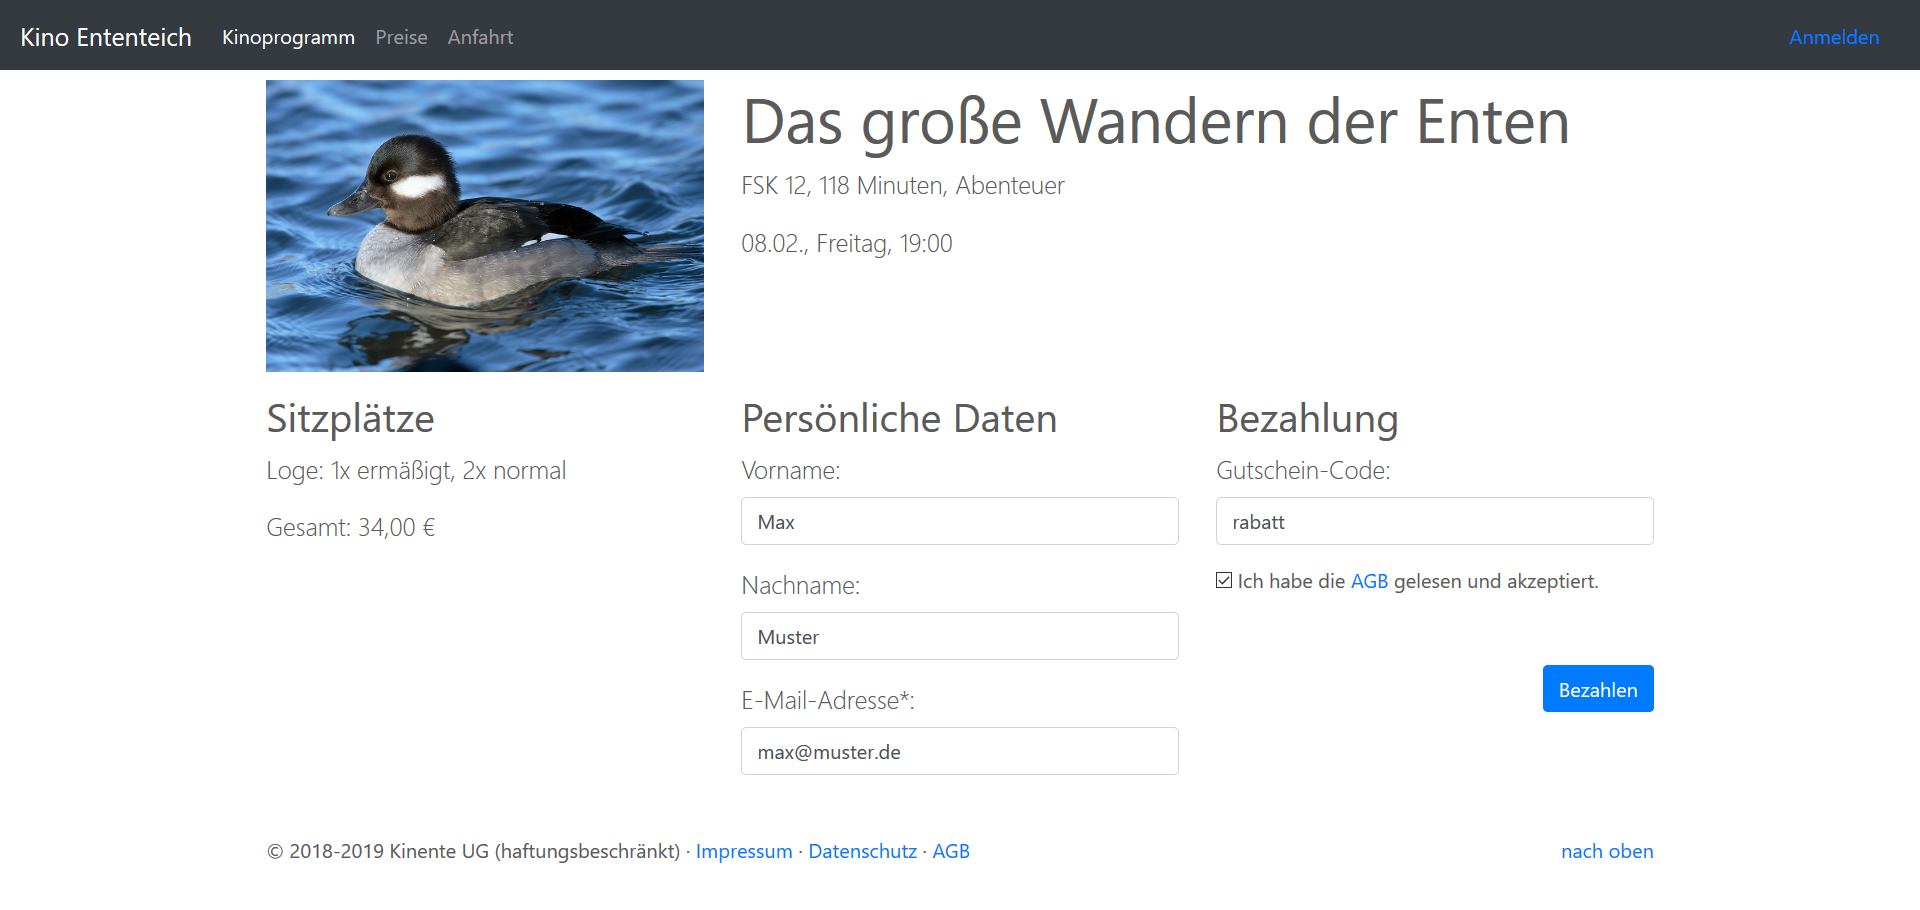
\includegraphics[width=0.95\textwidth]{img/screenshots/vorstellung03}
	\captionsetup{format=hang}
	\caption{Angabe weiterer Daten, die für den Buchungsvorgang relevant sind}
	\label{fig:vorstellung03}
\end{figure}

Die Daten werden dabei über \acs{URL}-Parameter weitergegeben.
Dies hat zwar den Nachteil, dass der Benutzer die Werte (z.B. den Gesamtpreis) theoretisch ändern könnte und dann andere Werte angezeigt bekommt.
Dies betrifft jedoch nicht die Sicherheit des Systems, da alle Überprüfung zwangsläufig zumindest im Back-End erfolgen müssen.
Am Beispiel des Preises würde dies bedeuten, dass der Benutzer zwar seine aktuelle Ansicht manipulieren kann, dennoch den korrekten Preis bezahlen muss.

Im oberen Bereich sieht der Benutzer nochmal allgemeine Informationen zur Vorstellung.
Des Weiteren erhält er eine Zusammenfassung zu seiner Sitzplatzauswahl mit dem Gesamtpreis.
Wenn sich der Benutzer entscheidet, die Sitzplätze verbindlich zu buchen, so wird im Hintergrund eine Nachricht an das Back-End gesendet.

Die Daten werden ähnlich wie beim Blocken eines Sitzplatzes in einem \acs{JSON}-Objekt gespeichert und mit einem \acs{AJAX}-Aufruf an das Back-End gesendet.

\begin{lstlisting}[language=JavaScript, caption={\acs{JSON}-Objekt für den Reservierungsvorgang}, label={lst:json_book}]
book = {paymentoption: "giftcard",
        verification: "rabatt",
        showId: 42,
        seats: [{id: 113, isReducedPrice: true},
                {id: 114, isReducedPrice: false},
                {id: 115, isReducedPrice: false}],
        customer: {firstname: "Max",
                   lastname: "Muster",
                   email: "max@muster.de"},
        sessiontoken: "TreevgQreNefpuUngHroreunhcgAvpugfTrznpug13"};
\end{lstlisting}

Neben den Informationen zur Vorstellung und den Sitzplätzen, wird auch noch die als Cookie gespeicherte Sitzungskennung mit angegeben.
Dies ist notwendig, damit eine Zuordnung zu den geblockten Sitzplätzen erfolgen kann.
Beim Auswählen des Sitzes wird der Sitzplatz für den Benutzer für eine gewisse Zeit geblockt.
Im Normalfall sind die Plätze beim Reservieren somit immer noch durch den Benutzer geblockt.
Durch die Angabe derselben Sitzungskennung, die auch beim Blocken verwendet wurde, ist es nun im möglich, dass im Back-End erkannt wird, dass der aktuelle Benutzer berechtigt ist, die geblockten Plätze zu reservieren.

Bei erfolgreicher Reservierung erhält man Informationen zur Reservierung, wie z.B. die Reservierungsnummer und die Tickets.
In diesem Fall kann auch die Bestätigung angezeigt werden, andernfalls erscheint eine Fehlermeldung.

Die Bestätigung enthält noch einmal alle Informationen zur Vorstellung, zur Anzahl der Sitzplätze und zum gezahlten Kaufpreis.
Unter einer kurzen Beschreibung zum weiteren Verlauf findet der Benutzer sein Ticket in Form eines \acs{QR-Code}s.
In diesem ist ein eindeutiger Verweis auf die Reservierung und somit auf alle Tickets gespeichert.
Der \acs{QR-Code} wird dabei unter Zuhilfenahme einer quelloffenen Bibliothek\footnote{\url{https://github.com/nayuki/QR-Code-generator}} erzeugt.

\begin{figure}[ht]
	\centering
	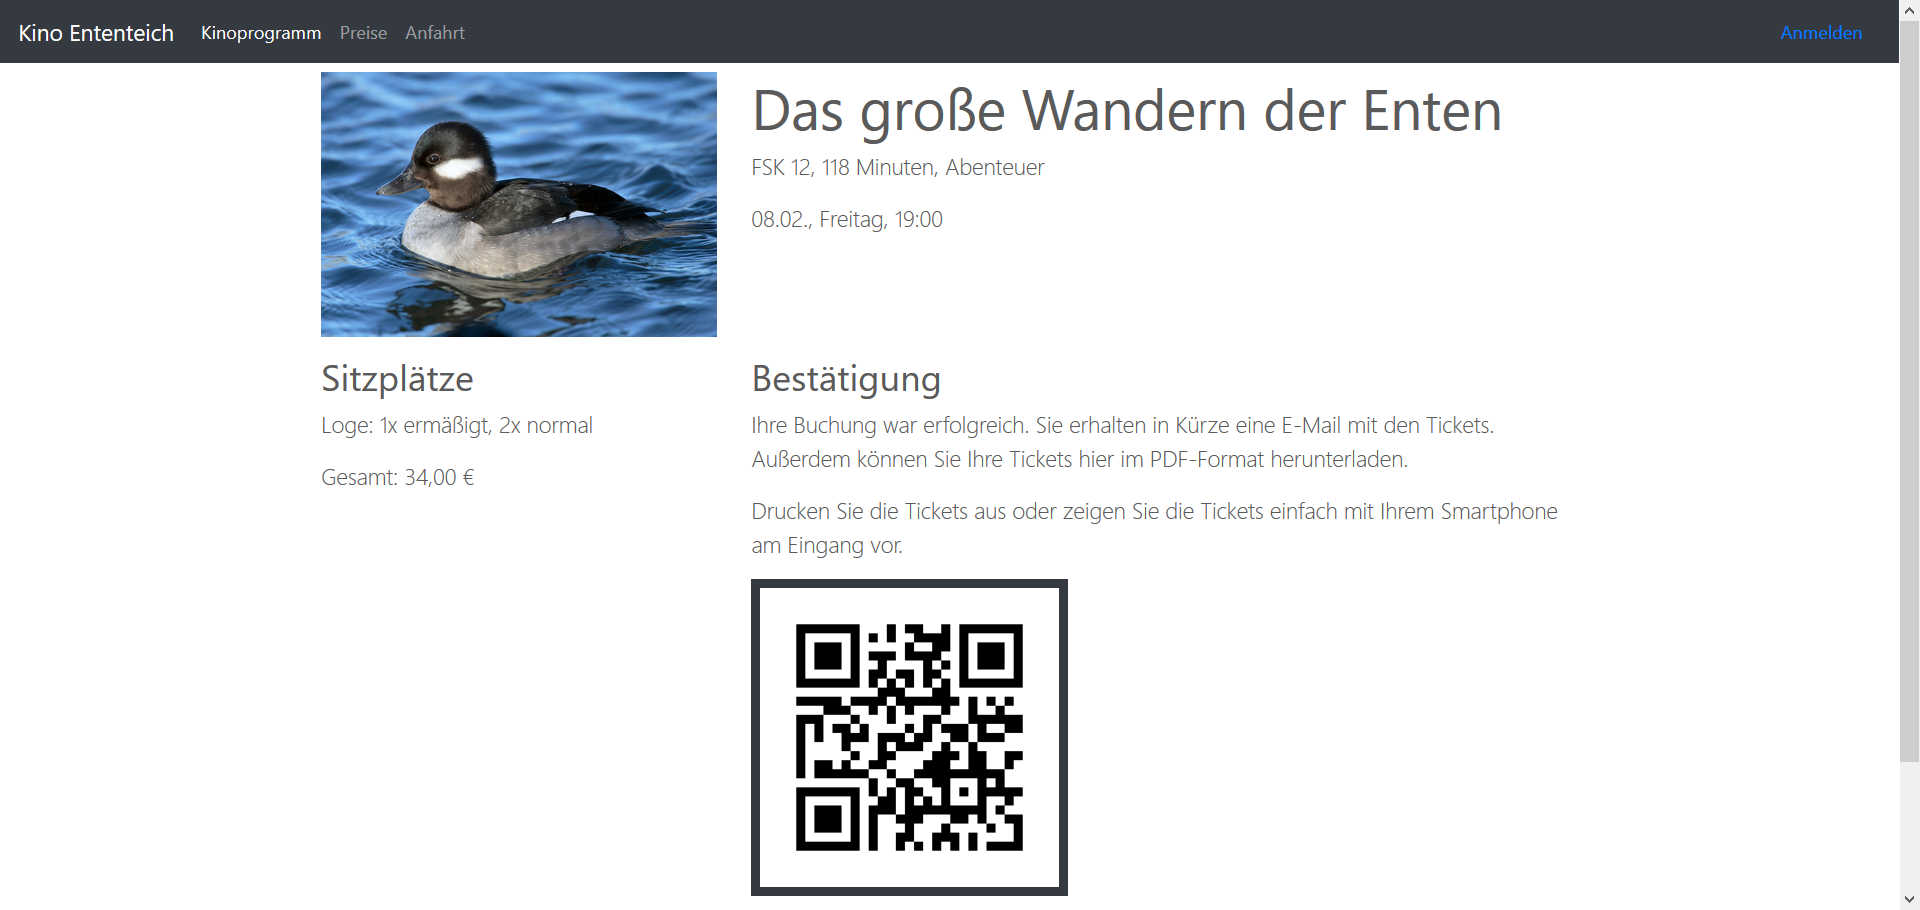
\includegraphics[width=0.98\textwidth]{img/screenshots/vorstellung04}
	\captionsetup{format=hang}
	\caption{Bestätigung einer Reservierung und Anzeige des \acs{QR-Code}s}
	\label{fig:vorstellung04}
\end{figure}

Im Kino kann an der Ticketkontrolle der \acs{QR-Code} gescannt und somit die Gültigkeit der Tickets überprüft werden.
Dadurch, dass ein \acs{QR-Code} für alle Tickets einer Reservierung steht, müssen sich die Benutzer, wenn sie mit mehreren Personen das Kino besuchen, keine Gedanken machen, wer welches Ticket erhält und die Tickets nicht untereinander verteilen. % TODO: move to design/planning?


% !TEX root =  master.tex
\chapter{Testen}
\label{sec:testen}
% !TEX root =  master.tex
\section{Softwarequalität}

Die Softwarequalität eines Programmes ist durch verschiedene Merkmale definiert. Zu diesen gehören Funktionalität, Portabilität, Zuverlässigkeit, Benutzbarkeit, Effizienz und Wartbarkeit. \footnote{\url{https://entwickler.de/online/agile/softwarequalitaet-so-misst-und-verbessert-man-software-114867.html}}
Ebenfalls geht es dabei um die Erfüllung der Erwartungen eines Benutzers an das Programm. In dem Fall, der für das Fach Fallstudie gestellten Anforderungen, handelt es sich um ein Kinoreservierungssystem,das über Frontend und Backend steuerbar sein soll.
Diese Qualitätsmerkmale sind wichtig einzuhalten, da sie die Zufriedenheit bei Kunden sowie Programmierer erhöhen, die Zuverlässigkeit der Software steigern, einen reibungsloseren Betriebsablauf gewähren, Kundenwünsche zuverlässiger erfüllt werden können, die Anforderungen besser und angepasster nach den Wünschen des Kundens erfüllt werden können und die Arbeitsprozesse beim Programmieren der Software effektiver gestaltet werden kann.
Im Allgemeinen ist Testen also nicht nur für den Kunden der Software wichtig, sondern auch für die Programmierer. 
Es bietet beiden Parteien Sicherheit um mit der Software zu arbeiten und diese zu verwalten. 
Dabei ist jedoch zu beachten, dass die Eliminierungen von Fehlern mittels Testen immer aufwendiger werden.
Je mehr Fehler bereits durch Tests abgedeckt wurden, desto teurer wird die Erhöhung der Testabdeckung. Der zu testende Code wird schwieriger zu testen und die Testerfolge sind nur noch kleinschrittig. Am Ende übersteigen die Kosten für das Kosten einer Codezeile deren Nutzen. Um für dieses Problem eine Lösung zu finden gibt es die das Qualitätsmanagement, es ist dafür da um ein Optimum aus Fehlerkosten und Fehlerverhütungskosten zu finden. Diese lassen sich zwar nicht genau bestimmen, aber können trotzdem durch Erfahrungswerte, Vergleichswerte und abschätzender Planung mithilfe von Soll- und Istwerten etwas eingegrenzt werden.\footnote{\url{http://www.enzyklopaedie-der-wirtschaftsinformatik.de/lexikon/is-management/Systementwicklung/Management-der-Systementwicklung/Software-Qualitatsmanagement}} Deshalb ist die Testabdeckung bei den meisten Projekten nicht auf ~100\% gefordert, sondern es wird sich auf einem niedrigeren Prozentsatz zwischen Kunde und Programmierer geeinigt. Für das Kinoreservierungsprogramm wird eine Codeabdeckung von ~60\% gefordert und wird in dem Kapitel \vref{sec:codeabdeckung} nochmal näher beschrieben.

% !TEX root =  master.tex
\section{Testverfahren}
Testen wird oftmals als Prozess, der aufzeigen soll, dass keine Fehler in dem Programmcode vorhanden sind, fehl verstanden. Im eigentlichen Sinne geht es dabei nicht darum zu zeigen, dass der Quellcode fehlerfrei ist, sondern das er Fehler enthält und nach diesen gesucht werden muss.\footnote{\url{http://www.knaupes.net/theorie-der-softwaretests/}}

\subsection{Testprinzipien}
Aufgrund dieser Definition für Testen müssen Ausgangsvoraussetzungen gegeben sein um eine möglichst umfangreiche Testabdeckung gewährleisten zu können. Zu diesen zählen das feststellen, ob der Quellcode genau die Anforderungen erfüllt und sonst auch keine weiteren Eventualitäten abdeckt. 
Ebenfalls sollte dabei genau dokumentiert werden, welcher Testfall bereits abgedeckt wurde. 
Da bei vielen unterschiedlichen Testfällen und einem größeren Testpensum der Überblick schnell verloren werden kann.
Des Weiteren müssen Testfälle reproduzierbar sein und es darf sich nicht um einzelnes Phänomen handeln. 
Einen Testfall zu generieren, der aber eigentlich gar nichts mit dem zu testenden Quellcode zu tun hat ist einerseits nicht möglich und andererseits nicht sinnvoll. 
Der aber wohl wichtigste Punkt, ob fachlich oder menschlich gesehen ist jedoch, dass der Tester nicht der Programmierer selbst sein darf.
Als Programmierer des Quellcodes besitzt man eine voreingenommene Meinung, der Quellcode hat genau einen Zweck und diesen erfüllt er für den Programmierer auch. 
Daher kann ein größerer Blickwinkel auf den Quellcode leider nicht gewährleistet werden und die Testfälle können nicht in hinreichender Genauigkeit generiert werden. 
Ebenfalls hat ein Tester auch keine leichte Aufgabe, da er sich in den Quellcode des Programmierers einarbeiten und diesen testen muss. 
Damit ist es aber noch nicht getan, da der Tester nun den Fehler weitergeben muss.
Das absichtliche Suchen nach Fehlern und dem Drang nach Perfektionismus durchzusetzen ist zwar notwendig aber kann schnell zu zwischenmenschlichen Konflikten führen. 
Deshalb ist sowohl auf Tester- und Programmierseite Vorsicht und auch Verständnis für die Aufgabe des Gegenparts geboten.

\subsection{Äquivalenzklassen}
Da selbst bei einem einfachen Test die möglichen Testfälle unmögliche viele werden können, kann durch die Äquivalenzklassen Abhilfe geschaffen werden. 
Diese Äquivalenzklassen verhalten sich gleich wie die getesten Eingabedaten, daher kann man davon aus gehen, dass diese Testfälle ebenfalls abgedeckt wurden. 
In diesem Sinne reicht es die Grenzfälle zu testen und bei allen anderen Möglichkeiten von einer äquivalente Verhaltensweise auszugehen.\footnote{\url{https://wr.informatik.uni-hamburg.de/_media/teaching/wintersemester_2010_2011/siw-1011-ehmke-tests-ausarbeitung.pdf}}  
Um dies mit einem Beispiel zu erläutern könnte man die Subtraktion von zwei Zahlen heranziehen. 
Wenn also die Subtraktion von Zahlen in einem Testfall funktioniert hat, dann kann man davon ausgehen, dass die anderen möglichen Testfälle mit Eingabedaten des gleichen Datenformates und Datentypes auch ein positives Ergebnis zurückgeben werden.

\subsection{Whitebox-Test und Blackbox-Test}
Bei beiden Testformen handelt es sich um eine Art den Quellcode auf seine Struktur, Design und Implementation zu testen. 
In einem Blackbox-Test hingegen ist der zu testende Code nicht bekannt und dies ist auch nicht erwünscht. 
Es handelt sich um eine einfache und billige Art und Weise das System zu testen. 
Der Programmierer erfordert keine Kenntnisse außer die Anforderungen an das System. Die möglichen Testmethoden sind Akzeptanz- und System-Tests, also Tests ob die Anforderungen des Benutzers und die Anforderungen an das System erfüllt wurden.  
Als Beispiel kann man sich einen Tester für ein Kinobuchungssystem vorstellen, der als Testfall das Buchen von Eintrittskarten heranzieht. 
Er besitzt weder Kenntnisse über das System, noch hat er eine konkrete Ahnung, welche Brennpunkte in dem System existieren und wird diese auch nicht explizit testen. 

Im Gegensatz dazu gibt es noch die Whitebox-Test, dabei handelt es sich um das Gegenteil eines Blackbox-Test.
Diese Methode ist im Gegensatz zu einem Blackbox-Test teurer und aufwendiger, aber führt zu einer genaueren Testabdeckung.
Der Tester hat detaillierte Kenntnisse über das System und hat Einblick in alle Ressourcen die den Quellcode betreffen.  
Die Testmethoden eines Whitebox-Testers sind Unit-Tests und Integrationstests, also Test auf die Verwendung von Codeabschnitten und einzelnen Codezeilen.
Das Beispiel für einen solchen Test wäre ein Tester, der jede Zeile eines Kinobuchungssystems auf Herz und Nieren testet. 
% !TEX root =  master.tex
\section{Technische Grundlagen der Tests}
\authorsection{\authorRF}

\subsection{JUnit}

\subsubsection{Allgemeines}

JUnit ist ein Java-Framework, welches vorwiegend zum automatisieren von Tests verschiedener Klassen und Methoden verwendet wird. \footnote{\url{https://junit.org/junit5/docs/current/user-guide/}}

Ein Test kann bei JUnit zwei Ergebnisse erzielen, entweder er schlägt fehl und wird mit rot markiert oder er läuft erfolgreich ab und wird grün markiert.
Bei den fehlgeschlagenen Tests wird jedoch noch weiter unterschieden. 
Es gibt sogenannte \enquote{Failures}, welche dadurch charakterisiert werden, dass nicht das erwartete Ergebnis beim Test aufgetreten ist.
Des Weiteren gibt es sogenannte \enquote{Error}, welche unerwartete Fehler sind, die während eines Tests auftreten können und somit den Test möglicherweise nicht vollenden lassen oder ein falsches Ergebnis hervorrufen.

Tests werden zudem als eigene Klassen realisiert, um sie vom Programmcode abzugrenzen und nicht vorm Kompilieren des Projektes entfernen zu müssen.

\subsubsection{Funktionsweise}

JUnit-Tests werden in Java mit Annotationen angekündigt und können mit diesen spezialisiert werden.
Standardmäßig wird ein Test mit \enquote{@Test} eingeleitet, danach folgt die eigentliche Test-Methode.
In der Test-Methode werden die zu testenden Klassen bzw. Methoden aufgerufen und mit Hilfe der \textit{assertEquals}-Methode getestet.
Hierbei wird ein erwarteter Wert bzw. ein erwartetes Objekt angegeben und diese mit den Ergebnissen der zu testenden Methoden auf Gleichheit geprüft.

Falls mehere Tests die selben Ausgangsdaten benötigen, kann mit Hilfe der \enquote{@BeforeAll}-Annotation einmalig zu Beginn bzw. mit \enquote{@BeforeEach} vor jeder Test-Methode eine Initialisierungsmethode eingeleitet werden, um die Ausgangsdaten zu erzeugen.
Gleichzeitig gibt es diese Annotationen auch nach den Tests, um bspw. Datenbankverbindungen erneut zu schließen. Diese Methoden werden mit \enquote{@AfterAll} und \enquote{@AfterEach} eingeleitet.

Außerdem können Tests überspringen werden, sofern sie mit \enquote{@Disabled} eingeleitet werden.
Dies hat einerseits Vorteile bei der Entwicklung, da so Tests schneller geprüft werden können, andererseits können so Tests auskommentiert werden sofern Bugs in den zu testenden Methoden vorhanden sind.


\subsection{Hamcrest}

Hamcrest ist wie JUnit ein Java-Framework, welches es leichter macht richtige Matcher-Objekte zu deklarieren. Jedoch ist Hamcrest als Zusatz zu JUnit zu betrachten und nicht als eigenständiges Test-Framework.
Dies ist ein großer Vorteil gegenüber dem Standard-Matcher von JUnit, da dieser allein mit der Gleichheit der Objekte arbeitet.
Somit is es einfacher komplette Kollektionen von Objekten auf Gleichheit zu testen oder komplexere Tests aufzustellen.

Hamcrest erlaubt es dem Nutzer zusätzlich auch eigene Matcher zu erstellen, welche das Testen erheblich erleichtern können.


% !TEX root =  master.tex
\section{Umsetzungen der Tests}

\subsection{Vorwort}

Das Kinoreservierungsprogramm befindet sich noch in Entwicklung, weshalb sich bei den Tests dafür entschieden wurde keine Testdatenbank zu erstellen.
Durch diese Maßnahme wurde Zeit eingespart, welche in die weitere Entwicklung einfließen konnte.
Jedoch sind die Autoren der Arbeit sich bewusst, dass sobald das Programm veröffentlich werden sollte, die Testdaten simuliert werden und somit keine Tests mit echten Daten in Bezug kommen sollten.

\subsection{Rollenverteilung}

Sofern Code und dazugehörige Tests von derselben Person bzw. Personengruppe entwickelt wird, entstehen oft im späteren Verlauf der Entwicklungsphase unerwartete Probleme. Diese Probleme entstehen dadurch, dass Entwickler oft ähnliche Werte zum Testen verwenden, wie sie bei der Entwicklung bedacht haben.
Eigenständige Tester jedoch betrachten Tests unvoreingenommenen und verwenden andere Werte, welche vom Entwickler möglicherweise nicht bedacht wurden.
Zudem zwingt es die Entwickler des Back-Ends dazu verständlichen Code bzw. dazugehörige Kommentare zu schreiben, da sonst die Entwicklung der Tests negativ beeinflusst werden kann.\footnote{\url{https://wr.informatik.uni-hamburg.de/_media/teaching/wintersemester_2010_2011/siw-1011-ehmke-tests-ausarbeitung.pdf}}

Dadurch, dass die Entwickler der Tests des Kinoreservierungsprogramms nur in moderatem Maß mit der Entwicklung des Back-Ends zu tun hatten, sind die Tests mit größtenteils unvoreingenommenen Ein- / Ausgabedaten entstanden.
Dies hat den Vorteil, dass diverse Szenarien betrachtet wurden, die bei der Entwicklung nicht bedacht worden sind.
Somit konnten Fehler des Back-Ends frühzeitig erkannt und behoben werden.


\subsection{Eigene Tests}

\subsubsection{Entitäten und Datentransferobjekte}

Nachdem in dem Projekt \acsp{DTO} (siehe Kapitel \vref{sec:dto}) verwendet werden, um die Daten aus der Datenhaltungsschicht der Drei-Schichten-Architektur in die Logikschicht zu transferieren, müssen diese an geeigneten Stellen von \acsp{DTO} zu Entitäten bzw. von Entitäten zu \acsp{DTO}  umgewandelt werden.
Dies geschieht mittels der \texttt{EntityToToHelper}- bzw. der \texttt{ToToEntityHelper}-Klasse. Diese Umwandlung wird für beide Klassen in eigenen Testklassen getestet.
Beide Testklassen sind grundlegend gleich aufgebaut, da beide erst Test-Entitäten bzw. Test-\acsp{DTO} mit den exakt gleichen Attributen erstellen.
Danach wird verglichen, ob das durch die Umwandlung entstandene Objekt die exakt gleichen Attribute besitzt. Zu sehen ist dies im Anhang \vref{src:entitytotohelpertest} anhand des Employee-\acsp{DTO}.
Im Code-Beispiel wird gezeigt, wie je ein \acs{DTO}-Objekt und ein Entitäts-Objekt erstellt wird und über \texttt{Set}-Methoden die exakt gleichen Werte übergeben werden.
In der nachfolgenden Test-Methode wird dann geprüft, ob bei der Eingabe von \texttt{NULL} kein Error entsteht, sondern \texttt{NULL} zurückgegeben wird.
Anschließend wird die Employee-Entität umgewandelt mit Hilfe der \texttt{EntityToToHelper}-Klasse und die jeweiligen Attribute überprüft, ob sie mit den Attributen des vorher erstellten Vergleichsobjekts übereinstimmen.
Dadurch werden alle \texttt{Getter}-Methoden getestet. Zudem werden durch das Erstellen der Objekte zu Beginn der Testklassen alle \texttt{Setter}-Methoden der Entitäts- und \acs{DTO}-Klassen mit genutzt und überprüft.

\subsubsection{JSON Konvertierung}

Das Überführen der Daten in das \acs{JSON}-Format ist ein wichtiger und entscheidender Schritt für die nahtlose Zusammenarbeit zwischen Front- und Back-End.
Deshalb wurde beim Testen der Konvertierungs-Klasse besonderen Wert auf Vollständigkeit gelegt. In der Testklasse wurde daher die Konvertierung für jeden einzelnen \acs{DTO}-Typen vorgenommen und überprüft.
Dies ist zwar nicht direkt notwendig, da die Klasse sich für jeden \acs{DTO}-Typen gleich verhält, aber erhöht jedoch die Sicherheit, dass keine unbemerkten Fehler bei diesem Schritt entstehen, ungemein.


\subsubsection{Eigene Werkzeuge}

Neben der \acs{JSON} Konvertierung wurden weitere Werkzeuge entworfen, um diverse Konvertierungen zu übernehmen.
Diese Werkzeuge befinden sich in der \texttt{Utils}-Klasse und erstrecken sich über Zeitkonvertierungen von Date-Objekten zu Strings, Informationen zum Datum oder Tag aus Strings herauslesen oder verschiedene Überprüfungen, ob die Buchung eines Sitzplatzes erfolgreich ist.
Zum Testen dieser Methoden reicht es aus vorher eigene Kalender-Objekte zu erstellen, diese umzuwandeln und mit vorher festgelegten Strings zu vergleichen.
Methoden zur Überprüfung, ob ein Sitz buchbar ist, wurden mit Hilfe von Sitz-Objekten und verschiedenen Zeitstempeln gebucht, so ist ein Sitz für eine aktuelle Vorstellung nicht, aber für zukünftige Vorstellungen buchbar.

\subsubsection{Ressourcen}
Die Ressourcen des Fachkonzepts, namentlich \texttt{ReservationResource, ShowResource, MovieResource}, wurden auch komplett auf ihre Funktionalität getestet.
Hierbei wurde darauf geachtet, dass jede Anfrage überprüft wird. Anhand der \texttt{ReservationResource} wird nachfolgend das Testen erklärt.

Zu Beginn des Tests werden alle zur Reservierung benötigten \acs{DTO}-Objekte angelegt, also ein Kunde, ein Buchungsobjekt sowie eine zu buchende Show.
Nachdem das Buchungsobjekt mit Hilfe der \acs{JSON} Konvertierung umgewandelt wurde, wird die \texttt{postTickets}-Methode der Ressource aufgerufen und der entstandene String übergeben.
Als Bestätigung, sofern das Buchen erfolgreich ist, wird ein Reservations-Objekt in Form eines \acs{JSON}-Strings übergeben. Dieser String wird wieder mit Hilfe der Konvertierungsklasse zurück umgewandelt in ein Reservations-Objekt.
Danach wird aus dem entstanden Reservations-Objekt die Id entnommen, um mit dieser geprüft, ob die Reservierung im System vorhanden ist. Dies geschieht mittels der \texttt{getReservationById}-Methode und hat ein Reservations-Objekt als \acs{JSON}-String als Rückgabewert.
Dieser \acs{JSON}-String wird erneut zu einem Reservierungs-Objekt umgewandelt, um das Objekt mit dem vorher aus der Buchung erhaltenen Objekt zu vergleichen. Damit wird sichergestellt, dass das Buchungs-Objekt auch alle Informationen enthält, die vorher abgegeben wurden.

Danach wird über die vorher ausgelesene Id die Reservierung gelöscht. Dies geschieht über die \texttt{deleteReservationById}-Methode und gibt wie die anderen beiden Methoden das gelöschte Reservations-Objekt als \acs{JSON} zurück.
Diese \acs{JSON} wird wie zuvor auch in ein Objekt umgewandelt und danach überprüft, sodass alle Informationen korrekt sind.
Zu Überprüfung, ob die Reservierung auch erfolgreich gelöscht wurde, wird am Ende des Tests überprüft, ob eine Reservierung unter der vorher erhaltenen Id vorhanden ist.

Zusätzlich wird in der \texttt{ReservationResource} das Blockieren und Deblockieren einzelner Sitze ausgeführt. Um dies zu Testen werden zwei Blockierungs-Objekte zu Beginn des Tests angelegt.
Diese bestehen aus einer eigenen Id, einem Sitz, der blockiert werden soll, einem Session Token und einer dazugehörigen Show, in der der Sitz blockiert werden soll.
Im Test wird so ein Sitz blockiert und wieder freigegeben, bei beiden Operationen wird ein Block-Objekt im \acs{JSON}-Format übergeben.
Diese Objekte werden anschließend auf ihre Gleichheit überprüft, um sicherzustellen, dass der blockierte Sitz mit dem freigegebenen Sitz übereinstimmt.

Die Tests der \texttt{ShowResource} und der \texttt{MovieResource} sind analog zum beschriebenen Test zu erklären.
Jedoch sind die beiden anderen Ressourcen auf das Auslesen von Daten spezialisiert und konnten somit leichter getestet werden.
Lediglich in der \texttt{MovieResource} befindet sich ein weiterer \texttt{Post} von Daten.
Dieser wurde ähnlich des \texttt{Posts} der Reservierung umgesetzt, mit dem Nachteil, dass ein Löschen eines Filmes im aktuellen Entwicklungsstand nicht möglich ist.
Dies muss per Hand nach dem Test gelöscht werden, da sonst ein Test-Film in der Datenbank steht.

\subsection{Codeabdeckung} 
\label{sec:codeabdeckung}
Für das Kinoreservierungsprogramm wurde bezüglich des Testens vorgeben, dass eine Codeabdeckung von 60\% erreicht werden soll.
Jedoch beziehen diese 60\% sich nur auf den eigenen logischen Code.

Durch die erstellten Tests werden $\sim$70,7\% des gesamten Codes der Datenhaltung und $\sim$65,9\% des gesamten Codes des Fachkonzepts abgedeckt.
Somit wurden die Vorgaben nicht nur erreicht, sondern überschritten.

Durch die Tests der verschiedenen Ressourcen des Fachkonzepts werden die dazugehörigen Services mit getestet.
Ein Testen der einzelnen Services im Back-End wurde durch die Komplexität des Projektes als nicht ökonomisch sinnvoll erachtet und aus zeitlichen Gründen nicht durchgeführt.
In Kapitel \vref{sec:konzept} wird der Zusammenhang der Fachkonzeptschicht mit der Datenhaltungsschicht erläutert.
Dieser Zusammenhang trägt auch zur Testabdeckung bei, wird jedoch durch die verwendete \acs{IDE} nicht dargestellt.
Somit kann jedoch nicht genau gesagt werden, um welchen Betrag sich die Testabdeckung des Datenhaltungs-Codes steigern würde.


% !TEX root =  master.tex
\chapter{Ausblick}
\label{c:ausblick}
\chaptermulitpleauthor{\authorRF}{\authorEJ, \authorSG, \authorNL}
% !TEX root =  master.tex
\section{Zukünftige Sprints und Backlog}

\subsection{Theoretischer Sprint 3}
\label{ssec:theoretischer_sprint}
\multipleauthorsection{\authorRF}{\authorEJ, \authorNL}
Die größte Neuerung des angedachten dritten Sprints ist die komplette Anbindung des Mitarbeiters.
Für einen Mitarbeiter sollen Vorname, Nachname, E-Mail-Adresse, Mitarbeiternummer und ein Passwort, in einer aktuellen Sicherheitsstandards genügenden Form (vgl. Kapitel \vref{sec:authentifizierung}), gespeichert werden.
Grundlagen dazu wurden bereits im vorhergehenden Sprint gelegt.
Eine Mitarbeiterrelation wurde in der Datenbank angelegt.
Teile der Businesslogik sind ebenfalls vorhanden, namentlich das Employee-\acs{DTO} und die Entität mit der zugehörigen Konvertierung.
Diese wurde bereits während der Testphase überprüft.

Eine Neuerung wäre eine spezielle Ansicht des Front-Ends angepasst an die Bedürfnisse der Mitarbeiter.
Hierzu zählen eine einfache Übersicht der aktuell laufenden Filme, eine simple und schnelle Suche nach Reservierungen und ein Kalendersteuerelement der nächsten 14 Spieltage im Kino. \\
Die Anordnung der Filme auf der Startseite des Mitarbeiters sollte nach dessen Belieben z.B. nach aktueller Uhrzeit erfolgen, sodass Primetime-Filme eine bestimmte Zeit vor Start des Blockbusters, aber auch zur jeweiligen Tageszeit eine passende Filmauswahl angezeigt werden. \\
Dies sollte den Buchungsvorgang vor Ort erheblich erleichtern und Teilzeitkräften sowie Ferienarbeitern den Einsteig in das System auch ohne eine lange Einarbeitungszeit ermöglichen. \\

Sobald ein Mitarbeiter eine Vorstellung ausgewählt hat, bekommen er und der Kunde vor Ort einen aktuellen Saalplan angezeigt.
Nachdem der Kunde nun seine gewünschten Sitze ausgewählt hat, beginnt der Bezahlvorgang.
Dieser erfolgt über ein bereits vorhandenes Kassensystem.
Beendet wird die Buchung schlussendlich durch das Ausdrucken der Kinotickets direkt an der Kasse.

Aufgrund der Bezahlung vor Ort muss die Mitarbeiteransicht in zweifacher Sicht geschützt werden.
Einerseits sollte das System nur innerhalb des lokalen Netzwerks verfügbar sein, andererseits ist eine Sicherheitsprüfung, in Form einer Authentifizierung, relevant, sodass kein Unbefugter Zugang zu den internen Bezahlsysteme erlangt.

Zusätzlich zu den genannten Hauptaspekten des dritten Sprints sollen kleinere Verbesserungen sowie Fehlerbeseitigungen durchgeführt werden.
Diese bestehen zum Beispiel aus der Verbesserung der Bestätigungsseite bei einer Online-Buchung.
Um die User Experience aufzuwerten und dem Benutzer ein besseres Erlebnis zu bieten, ist die Veränderung der Buchungsbestätigung im dritten Sprint nämlich unabdingbar.
Eine Einbindung der wie in dem Bild \ref{fig:ticket_phone} gezeigten Buchungsbestätigung gibt dem Benutzer weitere Informationen wie zum Beispiel Kinosaal, Reihe, Sitzplatz, Uhrzeit und Film, die in der aktuellen Version noch fehlen.

\begin{figure}[ht]
	\centering
	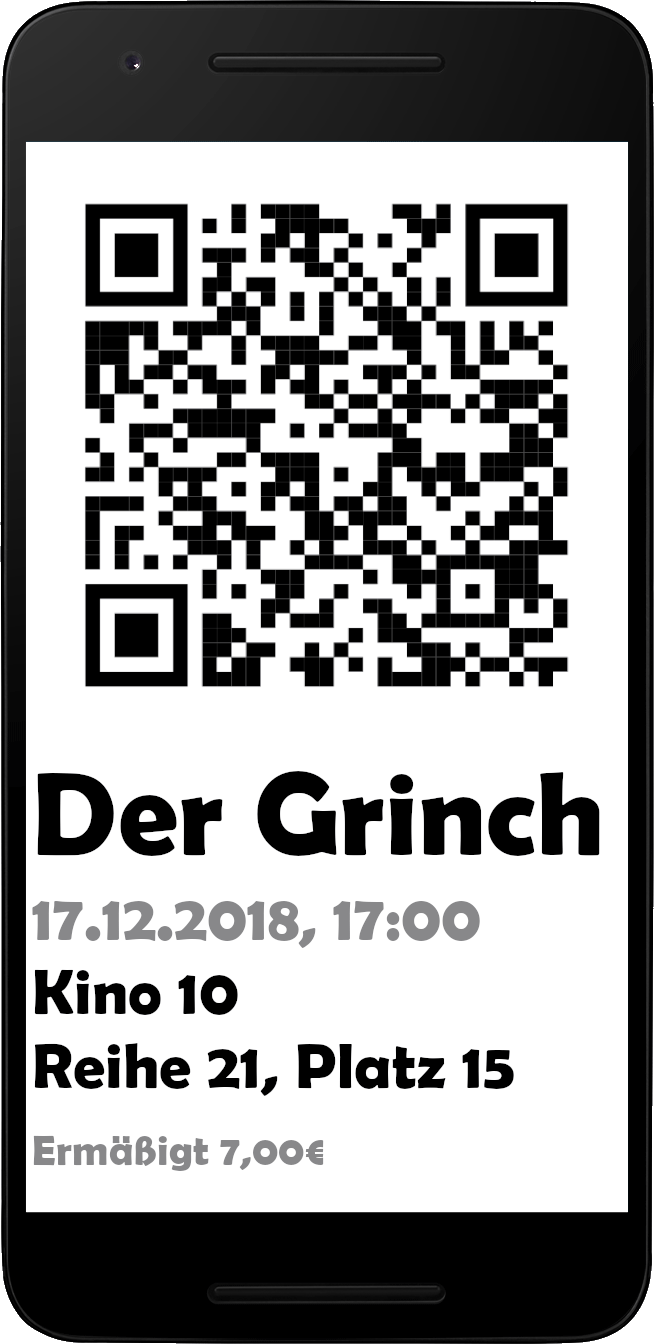
\includegraphics[width=0.2\textwidth]{img/ticket_phone}
	\captionsetup{format=hang}
	\caption{Digitales Ticket auf mobilem Endgerät}
	\label{fig:ticket_phone}
\end{figure}

Neben der Integration dieser Daten in das Handy-Ticket umfasst die Verbesserung der Bestätigungsseite aber auch das Ergänzen einer ausdruckbaren PDF-Datei für Kinobesucher, die die Möglichkeit, das Ticket digital auf dem Smartphone mitzuführen, nicht nutzen möchten.
Nach Möglichkeit wäre hier dann auch ein E-Mail-Versand der Bestätigung denkbar.

\subsection{Theoretischer Sprint 4}
\label{ssssec:sprint_benuterkonto}
\authorsection{\authorSG}
Durch den vierten Sprint soll dem Kinoreservierungssystem ein Benutzerkonto hinzugefügt werden.
Somit hätte der Kunde die Perspektive, sich in sein zuvor erstelltes Benutzerkonto einzuloggen.
Hier hätte er u.a. die Chance sein Passwort zu ändern und eine Übersicht über seine getätigtem Reservierungen zu haben.\
Hierbei bestünde dann die Aussicht, dass er auch eine getätigte Reservierung wieder stornieren kann.
Schlussendlich könnte man dem Kunden noch die Perspektive bieten, alle von ihm verfassten getätigten Rezensionen anzuzeigen.

Hierfür müssten lediglich neue \acs{REST}-Schnittstellen wie z.B. \jinline|reservation/customer| definiert werden, die für die Auswertung der getätigten Reservierungen verantwortlich wären.
Ebenfalls müssten im \jinline|CustomerService| die entsprechenden Methoden implementiert werden, sodass die aufgerufene Ressource das Ergebnis übermitteln kann.

Wie auch im dritten Sprint sollen hier kleine Verbesserungen sowie Fehlerbeseitigungen durchgeführt werden.

\subsection{Backlog}
\label{ssec:backlog}
\multipleauthorsection{\authorRF}{\authorEJ, \authorNL}
Für die langfristige Planung des Projektes wurden bereits Backlog-Items angelegt, die in späteren Sprints aufgefasst werden soll.

\subsubsection*{Gutschein}
\label{ssssec:gutschein}
Eine hohe Priorität hält dabei die Überprüfung und langfristige Speicherung der Gutscheincodes mithilfe der Datenbank inne.
Dabei sollen verschiedene Arten von Gutscheinen, sowie deren Ablaufdatum und vergangene Transaktionen gespeichert werden.

\subsubsection*{Bildformate und Dimensionen}
\label{ssssec:bildformatedimensionen}
Nachdem nicht jedes Filmplakat unbedingt im selben Format oder gar in den selben Dimensionen vorhanden sein wird, müssen diese Restriktionen im Endprodukt entfernt werden.
Hierbei ist vor allem zu beachten, dass Unternehmen eine einfache Bedienung der Software bevorzugen und somit beim Hinzufügen von Filmen im System die Bilder in diversen Formaten bereits mitgeben wollen.
Dabei sollten die Bilder für das Karussell sowie möglicherweise verschiedene Poster des Films einfach über eine Einrichtungsseite auf dem Front-End eingefügt werden können und durch das Back-End angepasst und in der Datenbank gespeichert werden.

\subsubsection*{Sitzplatzauswahl}
\label{ssssec:sitzplatzauswahl}
Die Darstellung der Sitze soll ebenfalls in einem zukünftigen Sprint angepasst werden, sodass einerseits Breite und Höhe eines Sitzes für die Darstellung mit gespeichert werden, andererseits aber auch Sitzflächen für Rollstuhlfahrer o.ä. ausgewiesen werden.

\subsubsection*{Kommunikation}
\label{ssssec:kommunikation}
Die Kommunikation zwischen Front- und Back-End muss erweitert werden.
Dabei sollten regelmäßige Abfragen das temporäre Speichern verschiedener Übergabeparameter ersetzen.

\subsubsection*{Zahlungsmöglichkeiten}
\label{ssssec:zahlungsmöglichkeiten}
Des Weiteren sollte ein breiteres Portfolio an Zahlungsmöglichkeiten das Benutzererlebnis verbessern und dem Kunden erlauben, ohne vorherigen Besuch des Kinos, online zu bezahlen.
Somit kann sichergestellt werden, dass den Kunden eine unverbindlichere und bequemere Art der Vorbestellung zu ermöglichen.
Als Alternative zu den weiteren Zahlungsmöglichkeiten, sollte die Option einer Reservierung (Bezahlung erst im Kino) gegeben sein.

\subsubsection*{Reservierungs-/Buchungsnummer}
\label{ssssec:reservierungsnummer}
Die Sicherheit der Tickets sollte ausgebaut werden.
Aktuell wird im \acs{QR-Code} lediglich die Reservierungs- bzw. Buchungsnummer gespeichert.
Da diese Reservierungsnummer der ID in der Datenbank entspricht, wird sie lediglich linear hochgezählt.
Ein böswilliger Angreifer könnte somit ziemlich einfach durch gezieltes Raten den Inhalt eines gültigen \acs{QR-Code}s erzeugen und unberechtigt Zutritt zu einer Kinovorstellung erhalten.
Durch eine zufällige in der Datenbank gespeicherte Nummer (Nonce), die neben der Reservierungsnummer in den \acs{QR-Code} mit einfließt, kann dies verhindert bzw. erschwert werden.

\subsubsection*{Stornieren und Verwalten}
\label{ssssec:stornieren_und_verwalten}
Einhergehend zur Reservierung, sollte eine Stornierung dieser, als auch eine Buchung möglich sein.

Um Reservierungen und Buchungen für einen passionierten Kinogänger einsehbar und verwaltbar (u.a. Stornierung) zu gestalten, wird ein Login eingerichtet.
Über diesen kann eine Personalisierung der Darstellung sowie Filmempfehlungen die User Experience verbessern.

% !TEX root =  master.tex
\section{Abgeschlossene und offene Ziele der Software}
\label{sec:ziele}
\subsection{Zieldefinition}
Das Ziel der Arbeit war es ein Kinobuchungssystem zu entwickeln, welches dem Benutzer ermöglicht eine Buchung durchzuführen.
Dieses Kinobuchungssystem sollte mit Hilfe der iterativen Vorgehensweise entwickelt werden.
Weitere Einschränkung des Entwurfs- und Entwicklungsprozesses war die Verwendung der Programmiersprache Java im Back-End (Vgl. \vref{sec:backend}) und den Entwicklungsprozess innerhalb von zwei Sprints und einem Bearbeitungszeitraum von zwölf Wochen abzuschließen.
Zudem sollten ca. 60\% des eigenen logischen Codes durch Tests abgedeckt werden. Dies bezieht sich lediglich auf das Back-End und den Businesscode des Projektes.

Unsere eigenen Ziele waren die Verwendung einer Datenbank, um die Voraussetzungen einer Drei-Schichten-Logik zu erfüllen.
Zudem sollte dies den Austausch von Daten im System erleichtern.

Weiterhin sollte es möglich sein einen kompletten Buchungsvorgang durchzuführen, d.h. von der Filmauswahl über die Vorstellungsauswahl sowie die Sitzplatzauswahl bis hin zur Buchung und deren Bestätigung zu gelangen.
Während des Buchungsvorganges soll dem Benutzer eine unverkennbare User Experience geboten werden, welche eine erneute Verwendung des Kinobuchungssystems begünstigt.

\subsection{Abgeschlossene Ziele}
Das vorliegende Kinosystem erfüllt alle gegebenen Zielvorgaben und überschreitet diese an diversen Stellen.
Das Back-End wurde innerhalb der zwei Iterationen um eine Datenbank sowie die geforderte Businesslogik erweitert. Darin beinhaltet ist eine Restriktion der mehrmaligen Buchung eines Sitzplatzes sowie das temporäre Blockieren eines online ausgewählten Sitzplatzes.

Im Front-End wurden alle geplanten Schritte der Buchung implementiert. Somit kann der Nutzer von der Filmauswahl bis zur Buchung ohne Unterbrechung die Funktionsweise eines Kinobuchungssystems in Anspruch nehmen. Dies wird jedoch limitiert durch eine vorgegebene Zahlungsmethode, welche nur vorher festgelegte Werte erlaubt.

Das Testen wurde, wie in Kapitel \vref{sec:testen} beschrieben, auch im Rahmen der Vorgaben erfüllt. Hierbei wurde das Ziel überschritten, da die zu testenden Klassen eine höhere Codeabdeckung als gefordert aufweisen.

Die eigenen Ziele wurden ebenfalls zum großen Teil erreicht. Das Verwenden einer Datenbank wurde mit Hilfe einer Postgres-Datenbank umgesetzt.
Hierzu wurden sämtliche von den Autoren festgelegten Attributen im Backend implementiert und für die weitere Verwendung bereitgestellt.
Durch die Implementierung von einem breiten Schnittstellen-Portfolio, die sowohl Speichern, Abrufen und Löschen mit Hilfe von \acs{REST}-Services ermöglichen, wird eine umfangreiche Kommunikation zwischen Front- und Back-End gewährleistet.
Somit wurde das Ziel einer klaren Trennung in Form der Drei-Schichten-Logik erreicht.

Ein weiteres, selbst gestecktes Ziel war es einen erfolgreichen Buchungsvorgang, wie in dem User-Journey (vgl. \vref{sec:user_journey}) beschrieben, zu durchlaufen.
Hierbei wurde im Front-End zusätzlich zur geplanten Filmauswahl ein Karussell mit aktuellen Blockbustern als Eye-Catcher implementiert.
Zudem wurde die Sitzplatzauswahl im Front- und Back-End gegenüber einer konventionellen Anordnung in Tabellenform durch ein Koordinatensystem ersetzt.
Hieraus ergeben sich diverse Möglichkeiten zu einer realitätsgetreuen Darstellung aller denkbaren zweidimensionalen Sitzplatzanordnungen sowie eine Skalierbarkeit der Saalgrößen bzw. Anzahl der Plätze.

Das Hauptziel der Arbeit, einen Sitzplatz einer Vorstellung nicht mehrmals zu verkaufen, wurde mit Hilfe des temporären Blockierens eines Sitzes gelöst. 
Genauer beschrieben wird der Ansatz in Kapitel \vref{ssssec:geblockt_durch_benutzer}.

Der Grundstein des theoretischen dritten Sprints wurde ebenfalls gelegt, indem ein Mitarbeiter im Back-End bereits implementiert wurde.


\subsection{Offene Ziele}

Zu den offenen Zielen, welche nicht in voller Gänze erreicht wurden, zählt die Sitzplatzdarstellung.
Diese sollte nach Plan auch eine Breite und Höhe in der Datenhaltung aufweisen, um jegliche Sitzarten (Sofas etc.) darstellen zu können.
Des Weiteren fehlt die Spezifikation für Rollstuhlplätze, diese werden in der aktuellen Version nicht dargestellt.
Jedoch ist das Potential für diese Änderungen im aktuellen System vorhanden, weshalb sie bei einem größeren Bearbeitungszeitraum auch erreicht worden wären.

Ein weiteres offenes Ziel ist die Umsetzung des Front-Ends als Single-Page-Application, hierbei wäre redundanter Datenaustausch verhindert worden.
Es wurde sich jedoch aufgrund Zeitmangels gegen eine frühzeitige Konvertierung des Front-Ends entschieden, um Ressourcen für Anpassungen im Back-End sowie der Tests frei zu halten.

Die unvergleichliche User Experience konnte zum jetzigen Zeitpunkt noch nicht erreicht werden, soll aber durch spätere Erweiterungen erreicht werden. 
Eine Fokussierung auf eine Eigenschaft der User Experience wäre dabei ein Weg dieses Ziel zu erreichen.
Dabei bietet sich das Vergnügen beim Benutzen des Systems hervorragend an, da dies eine der wichtigsten Eigenschaften bei einer Anwendung ist.

% !TEX root =  master.tex
\section{Kritische Reflexion und Bewertung}
\multipleauthorsection{\authorRF}{\authorEJ}

\subsection{Funktionalität und Qualität der Software}
\authorsection{\authorRF}

Das Front-End wurde mit Hilfe der Iterationsschritte erfolgreich nach den eigenen Wünschen umgesetzt.
Jedoch ist das aktuelle Design an diversen Stellen inkonsistent und weist sowohl farbliche als auch formtechnische Ungleichheiten auf.
Dies ist vor allem an der Sitzplatzauswahl zu erkennen, da die Darstellung nicht mit Design der sonstigen Website übereinstimmt.
Jedoch spiegelt das nicht das Endprodukt wieder und ist nur ein temporärer Makel.

Das Back-End wurde ebenso mit Hilfe der Iterationsschritte erfolgreich nach den eigenen Wünschen umgesetzt, jedoch weist es einige Schwächen auf.
Die Schwächen beziehen sich vorwiegend auf die Komplexität des Back-Ends im Bezug auf die Größe des gesamten Projekts.
So wurde das Drei-Schichten-Modell implementiert, was die Schwierigkeit beim Entwickeln und Benutzen erhöht hat.
Das in den Anforderungen als optional beschriebene Nutzen einer Datenbank hat somit einen großen Teil der Entwicklungszeit gekostet, welcher nicht für andere ebenfalls wichtige Entwicklungen oder Planungen genutzt werden konnte.

\subsection{Zusammenarbeit im Team}
\multipleauthorsection{\authorRF}{\authorEJ}

Die Gruppenarbeit ist allgemein positiv zu werten, so konnten alle Beteiligten Einblicke in möglicherweise unbekannte Bereiche gewinnen oder sich weiterbilden und den Kenntnisstand ausbauen.
Des Weiteren war die Motivation bei der Seminararbeit erhöht, da mit einem erfolgreichen und guten Projekt die Benotung derselbigen gut ausfallen sollte.

Dies führte auch dazu, dass ein großer Anteil der Gruppenarbeit auf individueller Basis entstanden ist und die Projektarbeit auf den aktuellen Stand gebracht hat, also ein funktionierendes Back-End mit einer Datenbank zur Datenhaltung sowie ein Front-End mit diversen nicht vorgegebenen Features, die als Alleinstellungsmerkmal angesehn werden können.
Jedoch wurde dadurch die Zusammenarbeit oftmals in den Hintergrund gerückt und es wurden Entscheidungen, welche vom Team demokratisch gefällt werden sollten, durch wenige Personen entschieden und eine Umsetzung angefangen. Dennoch wurden auch einige Prozesse in Teams erarbeitet, was oftmals das Verstehen des Sachverhalts erleichtert hat.
Durch das Übergehen verschiedener Personen bei Entscheidungen kam es auch schnell, u.a. auch durch fehlende Ambitionen, zu Demotivierungen, welche wiederum einseitige Arbeitsverhältnisse zur Folge hatten.

Trotzdem war die Arbeitsatmosphäre in den entstanden Gruppen und darüber hinaus recht entspannt, da im Team beschlossene Aufgaben in einem eigenen Arbeitstempo erledigt werden konnten und auch auf Schwächen einzelner Individuen Rücksicht genommen werden konnte.
% sollte man vielleicht nicht so drastisch formulieren -> "Gruppen-Abspaltung" etc. ist eher negativ konnotiert
Ferner wurden durch eine unsinnvolle Aufspaltung der Arbeit die gegebenen Ressourcen nicht erfolgreich genutzt und hätten das Projekt weiter fördern können.

Positiv hervorzuheben ist andererseits der erste Sprint, da hier erfolgreich als Team auf ein Ziel hin gearbeitet wurde und jeder seine individuellen Stärken einsetzen konnte.
Dies hatte einen schnellen Start zur Folge, der die vorher beschriebenen Problem erst ermöglicht hat.
Wobei hier eine klare Richtung des Projekts zu erkennen war, was allerdings durch ein fehlendes Projekt-Management im Team dazu geführt hat, dass die Energie und die Ambitionen nicht aufgegriffen wurden und in ein noch besseres und erfolgreicheres Projekt umgewandelt werden konnten.

Endgültig ist zu sagen, dass die Autoren als Team aus den Erfahrungen gelernt haben und nun in weiteren Projekten ein sinnvolles Projektmanagement umsetzen werden.
Dadurch sollte nicht nur die Motivation aller Team-Mitglieder gesteigert, sondern auch die Produktivität erhöht werden.
Diese Probleme und Lösungen sind das Ergebnis eines konstruktiven Feedbackgesprächs, welches am Ende des Projekts geführt wurde und bei dem jedes Mitglied seine Erfahrungen und Erkenntnisse teilen konnte.

% !TEX root =  master.tex
\section{Fazit zur Gruppen- und Seminararbeit}
\multipleauthorsection{\authorRF}{\authorEJ}

Durch die Gruppenarbeit konnte das Team viele positive Effekte einer Zusammenarbeit mitbekommen, zu diesen zählt einerseits die Leistungsstärke einer Gruppe.
Allein durch ein einzelnes Mitglied des Teams hätte niemals ein so fortgeschrittenes Modell eines Kinobuchungssystems erreicht werden können.
Andererseits konnte durch das Zusammenführen von verschiedenen Vorkenntnissen und Kompetenzen jedes Gruppenmitglied einen positiven Lerneffekt erlangen und dieses Wissen in die gestellte Aufgabe einbringen um ein Ergebnis zu erlangen, worauf jeder stolz sowie zufrieden sein kann.
Des Weiteren führt gegenseitiger Respekt zu einer positiven Atmosphäre, dabei stellt sich ein motivierendes und bildendes Lernklima ein.
Aufgrund wessen Entscheidungen innerhalb der Gruppe einfacher akzeptiert und mitgetragen wurden konnten.
Dieses Phänomen der Gruppendynamik ist nicht nur eine treibende Kraft für die gemeinsame Aufgabe, sondern bietet jeden einzelnen Gruppenmitglied Sicherheit und Zuversicht in sich selbst sowie andere.

Da jeder positive Effekt meistens auch noch einen negativen Beigeschmack hat auch diese Gruppenarbeit die möglichen Nachteile einer Zusammenarbeit aufgedeckt.
Einzelne Personen können eine sehr dominante Rolle innerhalb der Gruppe einnehmen und diese führen dabei zu einer Unterdrückung von Meinungen und erwürgen diese in keinem. 
Aus diesem Grund kann es schnell zu einem Gruppendenken kommen, die einzelnen Mitglieder denken nicht mehr selbst nach und folgen der Meinung anderer, obwohl es für das Problem wohl möglich noch bessere Lösungen gibt, die sonst noch keiner erwähnt hat.
Letztendlich ist die wohl komplexeste Aufgabe innerhalb eines Teams keine Spannungen entstehen zu lassen und falls sie doch entstehen sollten, diese bereitwillig zu beseitigen und sich vor keiner Konfrontation zu scheuen.
Dabei kann es schnell zu einer Minderung der Arbeitsqualität und Motivation kommen. 

Um einen bestmöglichen Effekt aus der Gruppenarbeit zu ziehen ist die Motivation einzelner Gruppenmitglieder, eine Koordination der Arbeitsressourcen, verschiedene Diskussionen für die Entscheidungsfindung sowohl das Vermeiden von Gruppendenken wichtig und notwendig.


Im Allgemeinen ist die Gruppenarbeit durch ein positives Arbeitsklima gekennzeichnet gewesen.
Allein durch die gesammelten Erfahrungen und Erkenntnisse konnten Probleme erkannt und Lösungen dazu erarbeitet werden.
Diese Probleme frühzeitig zu Erkennen und zu beheben ist nun für die Autoren der Arbeit einer der wichtigsten Aspekte einer Gruppenarbeit geworden.
Somit wurde durch ein Kinoreservierungssystem nicht nur der Gegenwert der Planung in einem Projekt, sondern auch die Wichtigkeit des Team-Managements und die Bedeutsamkeit der Kommunikation in Projekten mit mehreren Personen verdeutlicht.



% bibliography
\printbibliography[title=Literaturverzeichnis]
\cleardoublepage

% appendix
\appendix
\ihead{\appendixname~\thechapter}

\chapter{Abbildungen}
\begin{sidewaysfigure}
	\centering 
	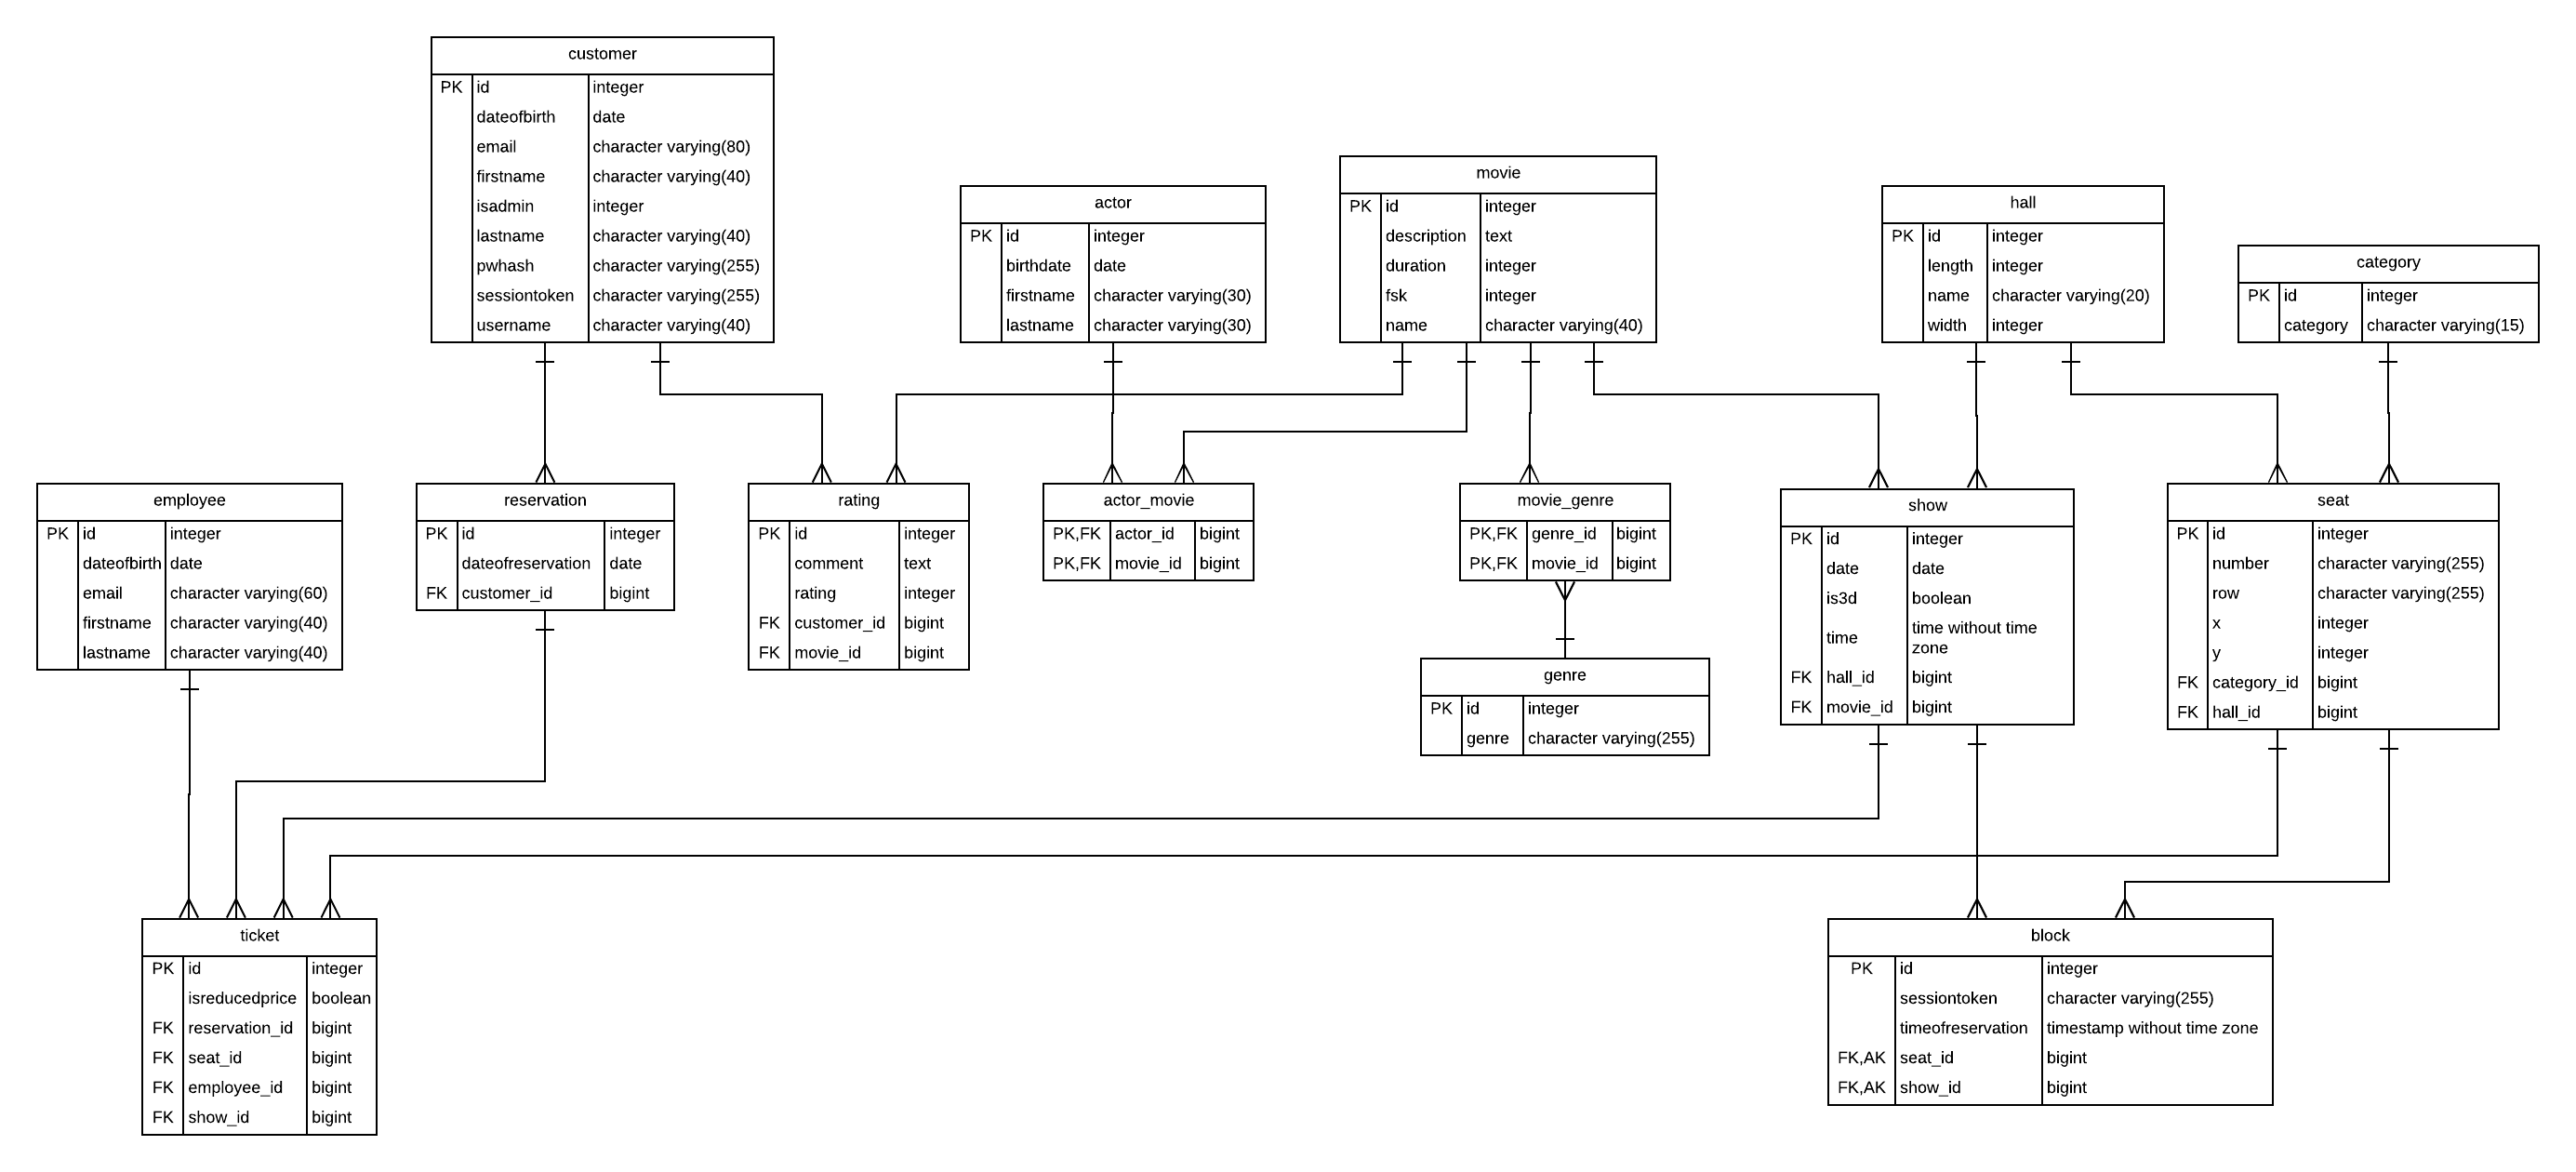
\includegraphics[keepaspectratio, width=1.0\textwidth, height=1.0\textheight]{img/ER-Modell}
	\captionsetup{format=hang}
	\caption{\acs{ER-Modell} der Datenbank}
	\small Quelle: eigene Darstellung mittels \url{https://www.lucidchart.com/}
	\label{fig:Anhang_ER-Modell}
\end{sidewaysfigure}

\chapter{Quellcode}
\begin{minipage}{\linewidth}
	\begin{lstlisting}[style=lstJava]
	public static MovieTo createMovieTo ( Movie entity, boolean withShow )
	{
	if ( null != entity )
	{
	MovieTo movieTo = new MovieTo();
	movieTo.setId(entity.getId());
	movieTo.setDescription(entity.getDescription());
	movieTo.setFsk(entity.getFsk());
	movieTo.setDuration(entity.getDuration());
	movieTo.setName(entity.getName());
	movieTo.setGenres(createGenreTos(entity.getGenres()));
	movieTo.setRatings(createRatingTos(entity.getRatings()));
	if ( withShow )
	{
	movieTo.setShows(createShowTos(entity.getShows(), false));
	} // end withSow
	movieTo.setActors(createActorTos(entity.getActors()));
	return movieTo;
	}  // end if null
	return null;
	}
	\end{lstlisting}
	\captionof{lstlisting}{Erstellen eines Movie-\acs{DTO} aus einer Movie-Entität mit Hilfe des eigen erstellten EntityToToHelper}
	\label{lst:EntityToToHelper_movie}
\end{minipage}

\begin{minipage}{\linewidth}
	\begin{lstlisting}[style=lstJava]
	public static Movie createMovieEntity ( MovieTo transferObject, boolean withShow )
	{
		if ( null != transferObject )
		{
			Movie movie = new Movie();
			movie.setId(transferObject.getId());
			movie.setActors(createActorEntities(transferObject.getActors()));
			movie.setDescription(transferObject.getDescription());
			movie.setFsk(transferObject.getFsk());
			movie.setDuration(transferObject.getDuration());
			movie.setName(transferObject.getName());
			movie.setRatings(createRatingEntities(transferObject.getRatings()));
			if ( withShow )
			{
				movie.setShows(createShowEntities(transferObject.getShows(), false));
			}
			movie.setGenres(createGenreEntities(transferObject.getGenres()));
			return movie;
		}
		return null;
	}
	\end{lstlisting}
	\captionof{lstlisting}{Erstellen einer Movie-Entität aus einem Movie-\acs{DTO} mit Hilfe des eigen erstellten ToToEntityHelper}
	\label{lst:ToToEntityHelper_movie}
\end{minipage}

% ewerkl.tex
% !TEX root =  master.tex

\clearpage
\chapter*{Ehrenwörtliche Erklärung}

Wir versichern hiermit, dass wir die vorliegende Arbeit
 mit dem Thema: \textit{\DerTitelDerArbeit} selbstständig verfasst und keine anderen als die angegebenen Quellen und
Hilfsmittel benutzt haben. Wir versichern zudem,
dass die eingereichte elektronische Fassung mit der gedruckten Fassung übereinstimmt.

\vspace{2cm}
Ort, Datum

\vspace{5mm}
\authorSG
\hfill \authorRF
\hfill \authorGP

\vspace{5mm}
\hfill \authorRF
\hfill \authorNL
\hfill

\end{document}
